

%% bare_jrnl.tex
%% V1.4b
%% 2015/08/26
%% by Michael Shell
%% see http://www.michaelshell.org/
%% for current contact information.
%%
%% This is a skeleton file demonstrating the use of IEEEtran.cls
%% (requires IEEEtran.cls version 1.8b or later) with an IEEE
%% journal paper.
%%
%% Support sites:
%% http://www.michaelshell.org/tex/ieeetran/
%% http://www.ctan.org/pkg/ieeetran
%% and
%% http://www.ieee.org/

%%*************************************************************************
%% Legal Notice:
%% This code is offered as-is without any warranty either expressed or
%% implied; without even the implied warranty of MERCHANTABILITY or
%% FITNESS FOR A PARTICULAR PURPOSE! 
%% User assumes all risk.
%% In no event shall the IEEE or any contributor to this code be liable for
%% any damages or losses, including, but not limited to, incidental,
%% consequential, or any other damages, resulting from the use or misuse
%% of any information contained here.
%%
%% All comments are the opinions of their respective authors and are not
%% necessarily endorsed by the IEEE.
%%
%% This work is distributed under the LaTeX Project Public License (LPPL)
%% ( http://www.latex-project.org/ ) version 1.3, and may be freely used,
%% distributed and modified. A copy of the LPPL, version 1.3, is included
%% in the base LaTeX documentation of all distributions of LaTeX released
%% 2003/12/01 or later.
%% Retain all contribution notices and credits.
%% ** Modified files should be clearly indicated as such, including  **
%% ** renaming them and changing author support contact information. **
%%*************************************************************************


% *** Authors should verify (and, if needed, correct) their LaTeX system  ***
% *** with the testflow diagnostic prior to trusting their LaTeX platform ***
% *** with production work. The IEEE's font choices and paper sizes can   ***
% *** trigger bugs that do not appear when using other class files.       ***                          ***
% The testflow support page is at:
% http://www.michaelshell.org/tex/testflow/



\documentclass[journal]{IEEEtran}
%
% If IEEEtran.cls has not been installed into the LaTeX system files,
% manually specify the path to it like:
% \documentclass[journal]{../sty/IEEEtran}





% Some very useful LaTeX packages include:
% (uncomment the ones you want to load)


% *** MISC UTILITY PACKAGES ***
%
%\usepackage{ifpdf}
% Heiko Oberdiek's ifpdf.sty is very useful if you need conditional
% compilation based on whether the output is pdf or dvi.
% usage:
% \ifpdf
%   % pdf code
% \else
%   % dvi code
% \fi
% The latest version of ifpdf.sty can be obtained from:
% http://www.ctan.org/pkg/ifpdf
% Also, note that IEEEtran.cls V1.7 and later provides a builtin
% \ifCLASSINFOpdf conditional that works the same way.
% When switching from latex to pdflatex and vice-versa, the compiler may
% have to be run twice to clear warning/error messages.






% *** CITATION PACKAGES ***
%
\usepackage{cite}
% cite.sty was written by Donald Arseneau
% V1.6 and later of IEEEtran pre-defines the format of the cite.sty package
% \cite{} output to follow that of the IEEE. Loading the cite package will
% result in citation numbers being automatically sorted and properly
% "compressed/ranged". e.g., [1], [9], [2], [7], [5], [6] without using
% cite.sty will become [1], [2], [5]--[7], [9] using cite.sty. cite.sty's
% \cite will automatically add leading space, if needed. Use cite.sty's
% noadjust option (cite.sty V3.8 and later) if you want to turn this off
% such as if a citation ever needs to be enclosed in parenthesis.
% cite.sty is already installed on most LaTeX systems. Be sure and use
% version 5.0 (2009-03-20) and later if using hyperref.sty.
% The latest version can be obtained at:
% http://www.ctan.org/pkg/cite
% The documentation is contained in the cite.sty file itself.


\usepackage{paralist}
\usepackage{caption}
\usepackage{subcaption}



% *** GRAPHICS RELATED PACKAGES ***
%
\ifCLASSINFOpdf
   \usepackage[pdftex]{graphicx}
  % declare the path(s) where your graphic files are
  % \graphicspath{{../pdf/}{../jpeg/}}
  % and their extensions so you won't have to specify these with
  % every instance of \includegraphics
  % \DeclareGraphicsExtensions{.pdf,.jpeg,.png}
\else
  % or other class option (dvipsone, dvipdf, if not using dvips). graphicx
  % will default to the driver specified in the system graphics.cfg if no
  % driver is specified.
  % \usepackage[dvips]{graphicx}
  % declare the path(s) where your graphic files are
  % \graphicspath{{../eps/}}
  % and their extensions so you won't have to specify these with
  % every instance of \includegraphics
  % \DeclareGraphicsExtensions{.eps}
\fi
% graphicx was written by David Carlisle and Sebastian Rahtz. It is
% required if you want graphics, photos, etc. graphicx.sty is already
% installed on most LaTeX systems. The latest version and documentation
% can be obtained at: 
% http://www.ctan.org/pkg/graphicx
% Another good source of documentation is "Using Imported Graphics in
% LaTeX2e" by Keith Reckdahl which can be found at:
% http://www.ctan.org/pkg/epslatex
%
% latex, and pdflatex in dvi mode, support graphics in encapsulated
% postscript (.eps) format. pdflatex in pdf mode supports graphics
% in .pdf, .jpeg, .png and .mps (metapost) formats. Users should ensure
% that all non-photo figures use a vector format (.eps, .pdf, .mps) and
% not a bitmapped formats (.jpeg, .png). The IEEE frowns on bitmapped formats
% which can result in "jaggedy"/blurry rendering of lines and letters as
% well as large increases in file sizes.
%
% You can find documentation about the pdfTeX application at:
% http://www.tug.org/applications/pdftex





% *** MATH PACKAGES ***
%
\usepackage{amsmath}
% A popular package from the American Mathematical Society that provides
% many useful and powerful commands for dealing with mathematics.
%
% Note that the amsmath package sets \interdisplaylinepenalty to 10000
% thus preventing page breaks from occurring within multiline equations. Use:
%\interdisplaylinepenalty=2500
% after loading amsmath to restore such page breaks as IEEEtran.cls normally
% does. amsmath.sty is already installed on most LaTeX systems. The latest
% version and documentation can be obtained at:
% http://www.ctan.org/pkg/amsmath





% *** SPECIALIZED LIST PACKAGES ***
%
%\usepackage{algorithmic}
% algorithmic.sty was written by Peter Williams and Rogerio Brito.
% This package provides an algorithmic environment fo describing algorithms.
% You can use the algorithmic environment in-text or within a figure
% environment to provide for a floating algorithm. Do NOT use the algorithm
% floating environment provided by algorithm.sty (by the same authors) or
% algorithm2e.sty (by Christophe Fiorio) as the IEEE does not use dedicated
% algorithm float types and packages that provide these will not provide
% correct IEEE style captions. The latest version and documentation of
% algorithmic.sty can be obtained at:
% http://www.ctan.org/pkg/algorithms
% Also of interest may be the (relatively newer and more customizable)
% algorithmicx.sty package by Szasz Janos:
% http://www.ctan.org/pkg/algorithmicx




% *** ALIGNMENT PACKAGES ***
%
%\usepackage{array}
% Frank Mittelbach's and David Carlisle's array.sty patches and improves
% the standard LaTeX2e array and tabular environments to provide better
% appearance and additional user controls. As the default LaTeX2e table
% generation code is lacking to the point of almost being broken with
% respect to the quality of the end results, all users are strongly
% advised to use an enhanced (at the very least that provided by array.sty)
% set of table tools. array.sty is already installed on most systems. The
% latest version and documentation can be obtained at:
% http://www.ctan.org/pkg/array


% IEEEtran contains the IEEEeqnarray family of commands that can be used to
% generate multiline equations as well as matrices, tables, etc., of high
% quality.




% *** SUBFIGURE PACKAGES ***
%\ifCLASSOPTIONcompsoc
%  \usepackage[caption=false,font=normalsize,labelfont=sf,textfont=sf]{subfig}
%\else
%  \usepackage[caption=false,font=footnotesize]{subfig}
%\fi
% subfig.sty, written by Steven Douglas Cochran, is the modern replacement
% for subfigure.sty, the latter of which is no longer maintained and is
% incompatible with some LaTeX packages including fixltx2e. However,
% subfig.sty requires and automatically loads Axel Sommerfeldt's caption.sty
% which will override IEEEtran.cls' handling of captions and this will result
% in non-IEEE style figure/table captions. To prevent this problem, be sure
% and invoke subfig.sty's "caption=false" package option (available since
% subfig.sty version 1.3, 2005/06/28) as this is will preserve IEEEtran.cls
% handling of captions.
% Note that the Computer Society format requires a larger sans serif font
% than the serif footnote size font used in traditional IEEE formatting
% and thus the need to invoke different subfig.sty package options depending
% on whether compsoc mode has been enabled.
%
% The latest version and documentation of subfig.sty can be obtained at:
% http://www.ctan.org/pkg/subfig




% *** FLOAT PACKAGES ***
%
%\usepackage{fixltx2e}
% fixltx2e, the successor to the earlier fix2col.sty, was written by
% Frank Mittelbach and David Carlisle. This package corrects a few problems
% in the LaTeX2e kernel, the most notable of which is that in current
% LaTeX2e releases, the ordering of single and double column floats is not
% guaranteed to be preserved. Thus, an unpatched LaTeX2e can allow a
% single column figure to be placed prior to an earlier double column
% figure.
% Be aware that LaTeX2e kernels dated 2015 and later have fixltx2e.sty's
% corrections already built into the system in which case a warning will
% be issued if an attempt is made to load fixltx2e.sty as it is no longer
% needed.
% The latest version and documentation can be found at:
% http://www.ctan.org/pkg/fixltx2e


%\usepackage{stfloats}
% stfloats.sty was written by Sigitas Tolusis. This package gives LaTeX2e
% the ability to do double column floats at the bottom of the page as well
% as the top. (e.g., "\begin{figure*}[!b]" is not normally possible in
% LaTeX2e). It also provides a command:
%\fnbelowfloat
% to enable the placement of footnotes below bottom floats (the standard
% LaTeX2e kernel puts them above bottom floats). This is an invasive package
% which rewrites many portions of the LaTeX2e float routines. It may not work
% with other packages that modify the LaTeX2e float routines. The latest
% version and documentation can be obtained at:
% http://www.ctan.org/pkg/stfloats
% Do not use the stfloats baselinefloat ability as the IEEE does not allow
% \baselineskip to stretch. Authors submitting work to the IEEE should note
% that the IEEE rarely uses double column equations and that authors should try
% to avoid such use. Do not be tempted to use the cuted.sty or midfloat.sty
% packages (also by Sigitas Tolusis) as the IEEE does not format its papers in
% such ways.
% Do not attempt to use stfloats with fixltx2e as they are incompatible.
% Instead, use Morten Hogholm'a dblfloatfix which combines the features
% of both fixltx2e and stfloats:
%
% \usepackage{dblfloatfix}
% The latest version can be found at:
% http://www.ctan.org/pkg/dblfloatfix




%\ifCLASSOPTIONcaptionsoff
%  \usepackage[nomarkers]{endfloat}
% \let\MYoriglatexcaption\caption
% \renewcommand{\caption}[2][\relax]{\MYoriglatexcaption[#2]{#2}}
%\fi
% endfloat.sty was written by James Darrell McCauley, Jeff Goldberg and 
% Axel Sommerfeldt. This package may be useful when used in conjunction with 
% IEEEtran.cls'  captionsoff option. Some IEEE journals/societies require that
% submissions have lists of figures/tables at the end of the paper and that
% figures/tables without any captions are placed on a page by themselves at
% the end of the document. If needed, the draftcls IEEEtran class option or
% \CLASSINPUTbaselinestretch interface can be used to increase the line
% spacing as well. Be sure and use the nomarkers option of endfloat to
% prevent endfloat from "marking" where the figures would have been placed
% in the text. The two hack lines of code above are a slight modification of
% that suggested by in the endfloat docs (section 8.4.1) to ensure that
% the full captions always appear in the list of figures/tables - even if
% the user used the short optional argument of \caption[]{}.
% IEEE papers do not typically make use of \caption[]'s optional argument,
% so this should not be an issue. A similar trick can be used to disable
% captions of packages such as subfig.sty that lack options to turn off
% the subcaptions:
% For subfig.sty:
% \let\MYorigsubfloat\subfloat
% \renewcommand{\subfloat}[2][\relax]{\MYorigsubfloat[]{#2}}
% However, the above trick will not work if both optional arguments of
% the \subfloat command are used. Furthermore, there needs to be a
% description of each subfigure *somewhere* and endfloat does not add
% subfigure captions to its list of figures. Thus, the best approach is to
% avoid the use of subfigure captions (many IEEE journals avoid them anyway)
% and instead reference/explain all the subfigures within the main caption.
% The latest version of endfloat.sty and its documentation can obtained at:
% http://www.ctan.org/pkg/endfloat
%
% The IEEEtran \ifCLASSOPTIONcaptionsoff conditional can also be used
% later in the document, say, to conditionally put the References on a 
% page by themselves.




% *** PDF, URL AND HYPERLINK PACKAGES ***
%
%\usepackage{url}
% url.sty was written by Donald Arseneau. It provides better support for
% handling and breaking URLs. url.sty is already installed on most LaTeX
% systems. The latest version and documentation can be obtained at:
% http://www.ctan.org/pkg/url
% Basically, \url{my_url_here}.




% *** Do not adjust lengths that control margins, column widths, etc. ***
% *** Do not use packages that alter fonts (such as pslatex).         ***
% There should be no need to do such things with IEEEtran.cls V1.6 and later.
% (Unless specifically asked to do so by the journal or conference you plan
% to submit to, of course. )


% correct bad hyphenation here
\hyphenation{op-tical net-works semi-conduc-tor}

%Commands
\newcommand\floor[1]{\lfloor#1\rfloor}
\newcommand\ceil[1]{\lceil#1\rceil}


\begin{document}
%
% paper title
% Titles are generally capitalized except for words such as a, an, and, as,
% at, but, by, for, in, nor, of, on, or, the, to and up, which are usually
% not capitalized unless they are the first or last word of the title.
% Linebreaks \\ can be used within to get better formatting as desired.
% Do not put math or special symbols in the title.
\title{Augmenting Amdahl's Second Law:  A Theoretical Model for Cost-Effective Balanced HPC Infrastructure for Data-Driven Science}
%
%
% author names and IEEE memberships
% note positions of commas and nonbreaking spaces ( ~ ) LaTeX will not break
% a structure at a ~ so this keeps an author's name from being broken across
% two lines.
% use \thanks{} to gain access to the first footnote area
% a separate \thanks must be used for each paragraph as LaTeX2e's \thanks
% was not built to handle multiple paragraphs
%

\author{
Arghya Kusum Das, %~\IEEEmembership{Member,~IEEE,}
Jaeki Hong, 
Kisung Lee, %~\IEEEmembership{Fellow,~OSA,}
Seung-Jong Park, %~\IEEEmembership{Life~Fellow,~IEEE}
Wooseok Chang\\
Department of Computer Science and Electrical Engineering, Center for Computation and Technology, Louisiana State University, Baton Rouge, LA, USA, 70803\\
Samsung Electronics Co., Ltd., 95, Samsung 2-ro, Giheung-gu, Yongin-si, Gyeonggi-do, S. Korea, 446711
% <-this % stops a space
\thanks{A. K. Das, K. Lee, and S.J. Park are with the Department
of Computer Science and Electrical Engineering, Center for Computation and Technology Louisiana State University, Baton Rouge, USA}
\thanks{J. Hong and W. Chang are with Samsung Electronics, S. Korea}
%GA, 30332 USA e-mail: (see http://www.michaelshell.org/contact.html).}% <-this % stops a space
%\thanks{J. Doe and J. Doe are with Anonymous University.}% <-this % stops a space
%\thanks{Manuscript received April 19, 2005; revised August 26, 2015.}
}

% note the % following the last \IEEEmembership and also \thanks - 
% these prevent an unwanted space from occurring between the last author name
% and the end of the author line. i.e., if you had this:
% 
% \author{....lastname \thanks{...} \thanks{...} }
%                     ^------------^------------^----Do not want these spaces!
%
% a space would be appended to the last name and could cause every name on that
% line to be shifted left slightly. This is one of those "LaTeX things". For
% instance, "\textbf{A} \textbf{B}" will typeset as "A B" not "AB". To get
% "AB" then you have to do: "\textbf{A}\textbf{B}"
% \thanks is no different in this regard, so shield the last } of each \thanks
% that ends a line with a % and do not let a space in before the next \thanks.
% Spaces after \IEEEmembership other than the last one are OK (and needed) as
% you are supposed to have spaces between the names. For what it is worth,
% this is a minor point as most people would not even notice if the said evil
% space somehow managed to creep in.



% The paper headers
\markboth{Journal of \LaTeX\ Class Files,~Vol.~14, No.~8, August~2015}%
{Shell \MakeLowercase{\textit{et al.}}: Bare Demo of IEEEtran.cls for IEEE Journals}
% The only time the second header will appear is for the odd numbered pages
% after the title page when using the twoside option.
% 
% *** Note that you probably will NOT want to include the author's ***
% *** name in the headers of peer review papers.                   ***
% You can use \ifCLASSOPTIONpeerreview for conditional compilation here if
% you desire.




% If you want to put a publisher's ID mark on the page you can do it like
% this:
%\IEEEpubid{0000--0000/00\$00.00~\copyright~2015 IEEE}
% Remember, if you use this you must call \IEEEpubidadjcol in the second
% column for its text to clear the IEEEpubid mark.



% use for special paper notices
%\IEEEspecialpapernotice{(Invited Paper)}




% make the title area
\maketitle

% As a general rule, do not put math, special symbols or citations
% in the abstract or keywords.
\begin{abstract}
Current compute technologies to analyze enterprise and scientific big data started demanding more processors, storage, and memory resources forcing a similar growth in the total computation cost. Consequently, the HPC system designers are facing relentless pressure to reduce the system cost while providing expected performance also for these data- and compute-intensive applications.  With this motivation, this paper proposes a simple, easy to use, additive model to optimize cost/performance by quantifying the system balance among CPU, I/O  bandwidth and size of DRAM in terms of both application characteristics and the hardware cost. Our performance model theoretically augment Amdahl's  second law for balanced system (Amdahl's I/O and memory number) and reveals that a balanced system needs almost 0.19GBPS I/O bandwidth, and almost 3GB of DRAM per GHz of CPU speed considering Intel Xeon processing architecture and current price trend in processor, storage and memory.
%The I/O- and memory-bound nature of data-driven scientific applications are posing several challenges to next generation HPC system designers as they strive for system balance with respect to processor speed, I/O bandwidth and memory while also maintaining a balance between performance and economy.  Augmenting Amdahl's design principles for balanced system, collectively known as \textit{Amdahl's second law} in the context of current big data analytic software (e.g., Hadoop, Giraph, etc.) and recent advances in hardware is relevant to design cost efficient HPC infrastructure for data-intensive scientific applications. This paper proposes a simple, easy to use, general purpose, additive model for cost/performance to quantify and optimize the system balance (among CPU, I/O  bandwidth and size of DRAM) in terms of both software characteristics as well as the current hardware cost. Our performance model reveals that a balanced HPC system needs almost 0.19GBPS I/O bandwidth, and almost 3GB of DRAM per GHz of CPU speed considering Intel Xeon processing architecture which is widely used by the HPC system designers. However, our model can be used for any given architecture. To the best of our knowledge, this is the first attempt to theoretically extend Amdahl's second law considering more degrees of freedom, such as, workload characteristics and hardware cost.

To substantiate our claim, we evaluate three fundamentally different cluster architecture, 1) a traditional HPC cluster called SupermikeII, 2) a regular datacenter called SwatIII, and 3) a novel micro brick based hyperscale system called CeresII. CeresII has 6-Xeon cores each running at 2GHz, 1-NVMe SSD with 2GBPS I/O bandwidth and 64GB DRAM, thus closely resembles to the optimum produced by our model. We evaluated these three clusters with respect to two widely used Hadoop-benchmark (terasort and wordcount) as well as our own genome assembler based on Hadoop and Giraph which serves as a real world example of data- and compute-intensive workload. CeresII outperformed all other cluster architecture for all the benchmark in terms of both execution time and cost/performance. For a large human genome assembly CeresII showed more than 85\% improvement over SuperMikeII and almost 40\% improvement over  SwatIII in terms of cost/performance.   
\end{abstract}

% Note that keywords are not normally used for peerreviewl
\begin{IEEEkeywords}
Cost to Performance, Balanced System, Hadoop, Giraph.
\end{IEEEkeywords}

% For peer review papers, you can put extra information on the cover
% page as needed:
% \ifCLASSOPTIONpeerreview
% \begin{center} \bfseries EDICS Category: 3-BBND \end{center}
% \fi
%
% For peerreview papers, this IEEEtran command inserts a page break and
% creates the second title. It will be ignored for other modes.
\IEEEpeerreviewmaketitle



\section{Introduction}
% The very first letter is a 2 line inial drop letter followed
% by the rest of the first word in caps.
% 
% form to use if the first word consists of a single letter:
% \IEEEPARstart{A}{demo} file is ....
% 
% form to use if you need the single drop letter followed by
% normal text (unknown if ever used by the IEEE):
% \IEEEPARstart{A}{}demo file is ....
% 
% Some journals put the first two words in caps:
% \IEEEPARstart{T}{his demo} file is ....
% 
% Here we have the typical use of a "T" for an initial drop letter
% and "HIS" in caps to complete the first word.
%%\IEEEPARstart{T}{his} demo file is intended to serve as a ``starter file''
%%for IEEE journal papers produced under \LaTeX\ using
%%IEEEtran.cls version 1.8b and later.
% You must have at least 2 lines in the paragraph with the drop letter
% (should never be an issue)
%%I wish you the best of success.

%%\hfill mds
 
%%\hfill August 26, 2015

\IEEEPARstart{C}{urrent} compute technologies for enterprise and scientific big data analysis are demanding more compute cycles per processor, with extreme I/O performance also required. At the same time, the hardware cost for storing and processing these big data is increasing linearly with the increase in volume and complexity of these data. Consequently, today's system designers are facing relentless pressure to reduce the system cost while providing the expected level of peroformance also. Complicating the scenario, the exponential growth of big data is rapidly changing the fundamental model of computation involved in high performace computating. A growing number of codes in both enterprise and scientific domain are being written using state of the art big data analytic software such as, Hadoop, Giraph which carefully consider data locality. 

%Traditional supercomputers focusing oly on doing calculation at blazing speed cannot produce expected level of performance. 
%A systematic and general approach is needed for these data-intensive applications both in terms of a computational model as well as cost-effective and balanced cyber infrastructure. The best practical approach till date was originally proposed by Jim Gray in 2000 (known as Gray’s Laws [2] [3]) where he stated, 1) Bring computations to the data, rather than data to the computations, and 2) The solution is in a scaled out architecture. With the increasing data size, the first law, which basically defines the locality-based model of computation utilizing lower network bandwidth, seems to govern the scientific big data analysis for next several years in future. For example, scientists are increasingly using Hadoop and other state of the art big data analytic software which carefully consider data locality. On the contrary, the second law, which defines the underlying distributed cyber infrastructure, needs to be clarified. 

As a consequence, most of the existing high performance  computing (HPC) clusters focusing only on tera to peta FLOP scale processing speed are found to be unbalanced (\cite{Amdahl:Workloadchang}, \cite{cluster:AmdahlBalancedBlade}) for data-intensive scientific applications either in terms of performance, or economy or both. Also, there is a long standing debate (\cite{scaleupscaleout:appuswamy} and \cite{scaleupscaleout:michael}) on scaled up versus  scaled out cluster architecture that these data- and compute-intensive applications require for better performance with optimized cost. 

As a matter of fact, the system characteristics of the data-intensive applications vary tremendously, especially because of varying nature and volume of data leading to no single solution in terms of underlying cluster archtecture. The problem becomes more complicated in a public cloud environment or HPC cluster where the application characteristics is not familier beforhand. In these scenarios, as an initial approach it makes sense to invest in a balanced cluster. Hardware vendors as well as cloud vendors (e.g., Amazon, Google, R-HPC, etc.) are investing huge amount of money for this. Millions of dollars are being spent for programs such as, NSF Cloud, XSEDE where several industries and universities collaborate to find such balanced architectures to drive the next generation cloud research. 

At this inflection point of HPC landscape, system designers must consider more degrees of freedom for cluster architecture than for existing HPC clusters which focus only on doing calculation at blazing speed. They must address such questions as: how much I/O bandwidth is required per processing core? How much memory is required to optimize the performance and cost?  Similar questions should be asked in the context of scaled up and scaled out architecture also. These complex performance and economic factors together motivate new design of HPC infrastructure, however, poses several challenges to the system designers who are striving for system balance in terms of processing speed, I/O bandwidth, memory, and the cost of the infrastructure. There is limited analytical studies which address the challenges in developing a cost-effective, balanced distributed cyber infrastructure to analyze large scale scientific big data.
 
With this motivation, this paper takes an initial attempt to theoretically augment Amdahl's second law for balanced system (in particular, Amdahl's I/O and Memory number) considering both the application characteristics as well as the price of hardware components. It proposes a simple additive model for cost/performance to quantify the system balance between CPU speed, I/O bandwidth, and size of DRAM in terms of software application characteristics and current trend in price. Our model does not assume any specific software framework or hardware technologies, rather, it provides an easy to use, general guideline for designing a balanced system. However, the outcome of the model (i.e., configuration of an optimal balanced system) suggest to use solid state drives (SSD) instead of hard disk drive (HDD) in a multicore machine. Assuming an equal distribution of I/O-  and compute work in a data-intensive application, our model suggests that a balanced HPC system needs almost 0.19-GBPS I/O bandwidth, and almost 3-GB of DRAM per GHz of CPU speed using Intel Xeon processor  and current price trend of different hardware. 

%We observed a convergence between our cost model and Amdahl's design principle. It is to be noted, we did not confine ourselves in proposing a performance model for any specific big data analytic software (e.g., Hadoop). Rather, we proposed a theoretical performance model for the underlying hardware only which is required by these big data analytic software for optimal performance. Thus, we are motivated to answer a more general question \textit{How does a next generation balanced HPC cluster should look like}

To substantiate our claim, we evaluate three fundamentally different cluster architecture as follows: 1) a traditional HPC cluster, called SuperMikeII (located at LSU, USA) that offers 382 computing nodes each with 16-Xeon cores, 1-HDD, and 32-GB DRAM, 2) a regular datacenter architecture, called SwatIII (located at Samsung, Korea) that has 128 nodes each with 16-Xeon cores, 4-HDD, and 256-GB DRAM and 3) a new MicroBrick-based architecture, called CeresII (also located at Samsung, Korea). Each CeresII node has  6-Xeon cores, 1-NVMe SSD  with 2-GBPS I/O bandwidth and 6-GB DRAM per node, thus closely resembles to the optimum produced by our model. We evaluated these three architectures with respect to three different benchmark applications. Two of them are widely  used benchmark Hadoop applications (e.g., TeraSort and WordCount) and the other one is our own benchmark genome assembler developed atop Hadoop and Giraph which serves as a good real-world example of a data-, compute- and memory-intensive workload. For all the three benchmark evaluation, CeresII, with the most optimum configuration outperformed the others in terms of both performance and cost/performance when using same amount of processing cores as SuperMikeII and SwatIII across the cluster, and significantly less (almost half) DRAM than SwatIII. 

The rest of the paper is organized as follows: Section-\ref{sec:RelatedWork} describes the prior work relate to our current effort. Section-\ref{sec:Motivation} describes our mtivation for this study. In Section-\ref{sec:AmdahlGray}, we discuss Amdahl's second law in details. Section-\ref{sec:Model} describes the proposed model. Then, in Secton-\ref{sec:ExperimentalTestbed} shows the details of our experimental tesbeds and classifies those using our proposed model. Section-\ref{sec:EvalMethod} describes the evalutation methodology for these clusters, i.e., the details of the software and benchmark that we used in our evaluation. In Section-\ref{sec:Result} we discuss the experimental result. Finally Section-\ref{sec:Conclusion} concluded the paper. 

\section{Related Work} \label{sec:RelatedWork}
Numerous studies have been performed evaluating the performance implication of different big data analytic software on different types of hardware infrastructure. We categorize these existing studies into three different classes such as 1) experimental evaluation of different cluster architecture for big data software, 2) simulation and analytical performance modeling of big data software, and 3) system characterization using Amdahl's second law which is the most relevant to our current effort. In this section we discuss the previous works done in these three categories.

\subsection{Experimental evaluation of different cluster architecture for big data software.} 
Kang \cite{ssdhdd:kang} compared the execution time of sort, join, WordCount, Bayesian, and DFSIO workloads using SSD and HDD and obtained better performance using SSD. Wu \cite{ssdhdd:wu} found that Hadoop performance can be increased almost linearly with the increasing fraction of SSDs in the storage system. They used the TeraSort benchmark for their study. Additionally, they also showed that in an SSD-dominant cluster, Hadoop's performance is almost insensitive to different Hadoop performance parameters such as block-size and buffer-size. Moon \cite{ssdhdd:moon} showed a significant cost benefit by storing the intermediate Hadoop data in SSD, leaving HDDs to store Hadoop Distributed File System (HDFS \cite{fw:hdfs}) data. They also used the TeraSort benchmark in their study. A similar result can be found in the study by Li \cite{ssdhdd:li} and Krish \cite{ssdhdd:krish} where SSDs are used to store temporary data to reduce disk contention and HDDs are used to store the HDFS data. They all reached the same conclusion as Moon \cite{ssdhdd:moon}.  Tan \cite{ssdhdd:tan} also reached the similar conclusion for two other workloads including a Hive workload and an HBase workload. 

Michael \cite{scaleupscaleout:michael} investigated the performance characteristics of the scaled out and scaled up architecture for interactive queries and found better performance using a scaled out cluster. On the other hand, Appuswamy \cite{scaleupscaleout:appuswamy} reached an entirely different conclusion in their study. They observed a single scaled up server to perform better than a 8-nodes scaled out cluster for eleven different enterprise-level Hadoop workloads including log-processing, sorting, Mahout machine learning, etc. However, these studies do not provide any quantitative measure for scale up or scale out.  

However, an older study by Kung \cite{Balance:kung1986memory} can shed light on feasibility of the scaling up approach. Kung analyzed several HPC problems and theoretically showed that the memory needs to be increased exponentially to restore the balance of the system when the number of processors is increased by a certain factor. For example, best known external sorting algorithm needs the local memory to be increased by an exponent of $\alpha$ when number of processors are increased by a factor of  $\alpha$ (i.e., $M_{new} = M_{old}^{\alpha}$) to restore the balance of the system. Although this study is not directly related to this paper, some of the problems considered in \cite{Balance:kung1986memory} constitutes the core part of today's big data analytic framework. For example, Hadoop uses the similar external sorting in its shuffle phase. Hence, from the perspective of balanced system design arbitrary scaling up the size of DRAM is possibly not a feasible option. Rather, the amount of RAM should be decided based upon cost.

\subsection{Simulation and analytical performance modeling of big data software}
Simulation and analytical models are widely used for predicting performance of different big data software (mainly Hadoop) and analyzing design trade-offs in a large number of hardware domains. 

At the border level, all simulators generate virtual Hadoop MapReduce jobs and tune different hardware and software parameters in a simulated environment mostly using prior experiences or trial-and-error to optimize the performance of some parts of the Hadoop framework or a given Hadoop job. For example, HSim \cite{Simulator:liu2013hsim} mainly focused on the Hadoop job parameters to optimize the performance of the entire job. SimMR \cite{Simulator:verma2011play} on the other hand focus on simulating the Hadoop task scheduling algorithms. MRSim\cite{Simulator:hammoud2010mrsim} and MRPerf \cite{Simulator:wang2009simulation} unified all these aspects in a single simulator. They simulate the hardware environment using discrete event simulator packages such as,  SimJava, GridSim, NS2, etc. Then  they execute the fake Hadoop job on a small subset of data to predict the performance. Given prior experience, simulators can predict hardware alternative, thus capable to save huge cost comparing to experimental evaluation on real hardware discussed before. However, most of these simulators comes with lots of overhead. They are time and resource consuming and often fail to assess the real system characteristics in the presence of huge volumes of big data. Furthermore, the trial-and-error method of performance optimization considering broad range of available hardware infrastructure with more $200$ Hadoop parameters is challenging and most of the time unreliable.

On the other hand, analytical models for abstract away several performance parameters and predict the performance of a Hadoop job mainly using single or multi layer queuing network. For example, Viana \cite{Model:vianna2013analytical} model the pipeline parallelism of a Hadoop job using queuing network to predict the performance of the job.  Wu \cite{Model:wu2015exploring} proposed a layered queue network model to predict the performance of a Hadoop job in a cloud environment. In a recent work Ahn \cite{Model:ahn2015analytical} proposed a queuing theory model to predict the performance of Hadoop job atop different storage technologies, i.e, HDD and SSD. Krevart \cite{Model:krevat2010applying} computed the I/O complexity of the Hadoop job for data-intensive applications and proposed a model to quantify the hardware resource wasted by Hadoop.  They (Krevart) shouted for improving the big data analytic software.

\subsection{System characterization using Amdahl's second law }
Computer scientist Gene Amdahl postulated several design principles for a balanced system design collectively known as Amdahl's Second Law. He stated a balanced system needs 1-bit of sequential I/O per second (Amdahl's I/O number), and 1-byte of memory (Amdahl's memory number) per CPU instruction per second. Jim Gray \cite{Amdahl:RuleofThumbgray2000rules} in 2000 revised Amdahl's second law by suggesting to measure the instruction rate and I/O rate on the relevant workload. We will discuss it in more details later in Section-\ref{sec:AmdahlGray}.
%Based upon these studies, Dobos and Szalay \cite{Amdahl:Graywulfdobos2013graywulf} proposed a balanced system called GrayWulf for data intensive computing that won the storage challenge in SuperComputing 2008. 

Bell and Gray \cite{Amdahl:PetascaleBell2005petascale} also classified the existing supercomputers based upon Amdahl's second law to clarify the future roadmap of the HPC architecture. Chang  \cite{Amdahl:Workloadchang} used Amdahl's second law to better understand the design implications of data analytic systems by quantifying workload requirements.  Cohen \cite{Balance:cohen2009applying} applied Amdahl’s second law to study the interplay between processor architecture and network interconnect in a datacenter. 

Szalay \cite{cluster:AmdahlBalancedBlade}, used Amdahl's I/O and memory numbers to propose an energy efficient balanced cluster architecture Amdahl’s bananced blades. \cite{cluster:AmdahlBalancedBlade} used SSD and low power processors (such as, Intel Atom, Zotac etc) to achieve the system balance. In this study, the authors ignored the CPU micro architecture and simplified the Amdahl's I/O and Memory number by dividing the I/O bandwidth (bit/s) and size of DRAM (GB) respectively by CPU-speed (GHz). The cluster architecture was balanced as the simplified Amdahl's I/O number was close to unity. In a recent study \cite{Balance:zheng2014hadoop} Zheng evaluated a similar architecture as Amdahl's balanced blade for Hadoop applications and showed Atom processor is the system's bottleneck  %In a recent work, Liang [25] applied Amdahl’s second law for performance characterization of two different state of the art big data analytic software (e.g., Hadoop and DataMPI).  

\section{Motivation: Architectural (Im)balance in Traditional HPC Cluster and Recent trend in Hardware} \label{sec:Motivation}
There are several important reasons to model the performance for a cloud application on a given processor architecture using analytical approach. The most common one is evaluating alternative hardware configurations.
\subsection{Network Architecture}
Traditional HPC clusters uses a hierarchy of switches with a fat tree model of connectivity. This approach typically uses layered architecture. The hosts or servers are connected to the bottom layer, called access layer which is then aggregated to an intermidiate layer of switches, called edge layer or leaf. The edge layer switches are then connected to the top layer switches, called core layer or spine where the actual bandwidth of the network is scaled. To prevent over subscription, the link speeds got progressively higher from access layer to leaves to spine starting from only few Mbps to several Gbps. This architecture may suffer from bottleneck issues thereby introduces architectural imbalance in the modern datacenter or cloud infrastructures as the bandwidth of the host adapter is increasing in an outstanding pace (an observation by Cohen [24]). Furthermore, to accomodate many servers with fewer switches (thus, reducing the cost of the network) a blocking is used which again limits the performance of big data genomic applications which demand more bandwidth.

As an alternative, the simple Clos based architecture is gaining popularity where all the lower layer switches (i.e., leaf) are connected to all the top layer switches (i.e., spine) using a full mesh topology, thus achieving a non-blocking model using inexpensive devices. The data-intensive applications based of Hadoop or Giraph, which transmits huge amount of data over network in different phases of computation, can use more bandwidth from this all-to-all connection model.

\subsection{Storage Architecture}
The performance of any system is traditioanlly constrained by the I/O subsystem. So is the traditional HPC cluster which are normally equipped with only one hard disk drive. Over the span of last 10 years the the hard disk speed is improved by only twice from 7000RPM to 15000RPM. Consequently, the I/O throughput increased from 80MB/s to 150MB/s. At this rate, to read just a 1TB hard disk takes almost two hours. In real world scenario, where a huge amount of data is read/write from/to the local disk the performance may be even worse. So, in many state of the art data center cluster and cloud infrastructure the data is stripped across multiple smaller disks to improve the I/O throughput.

Alternatively, the SSDs can be used. It uses the similar flash memory that is used in memory subsystem, thus increases the per-disk I/O throughput by almost 4-times than an HDD. Current SSDs offer almost 550MB/s I/O throughput in a moderate cost while maintaining considerable storage capacity. Due to the high bandwidth of SSDs, the most intuitive approach to build a high performance cluster is to use multiple SSDs with high end processors. However, the disk controllers are found to

\subsection{Memory Architecture}
With the introduction of DDR (Double Data Rate) technology the memory bandwidth has been improved significantly because it reads one word of data during the positive edge and one word during the negative edge of the processor clock pulse. Most of the current HPC cluster as well as the computation clusters use either DDR2 or DDR3 RAM (random access memory or, simply main memory) modules. There is hardly any difference among current clusters (including traditional HPC clusters and datacenters) in terms of memory architecture or processormemory communication model. 

However, for improved performance, suffcient memory should be provided to the cluster that can hold the required computation in conjunction with the big data. Furthermore, more memory improves the caching effect which again improves the applications’ performance. However, the main memory is costly which makes the job of building the balanced system complicated. Again, the SSD is nowadays increasingly considered as a new layer between memory (Since they use similar flash arrays as RAM) and storage due to its increased I/O bandwidth which is changing the designer’s approcah towards a balanced system. 

\section{Amdahl's Second law, Gray's Ammendment, and Their Limitations} \label{sec:AmdahlGray}
\subsection{Original Form of Amdahl's Second Law}
Computer scientist Gene Amdahl postulated several design pronciple in late 1960 to make a balanced system. As mentioned earlier, these design principals are collectively known as Amdahl’s second law  which are as follows:
\begin{enumerate}
\item Amdahl’s I/O Law: A balanced computer system needs one bit of sequential I/O per second per instruction per second. From this point we will mention this law as Amdahl’s I/O number. Alternatively, Amdahl's I/O number of a balanced system can be expressed as $0.125$ GBPS/GIPS (by changing in conventional units).
%\begin{equation} \label{eqn:AmdahlIoNo}
%Amdahl's I/O Number = \frac{I/O Bandwidth (bit/s)}{CPU Speed (GIPS)} = 1
%\end{equation}
\item Amdahl’s memory Law: A balanced computer system needs one byte of memory per instruction per second. IFrom this point we will mention this law as Amdahl’s memory number.
%\begin{equation} \label{eqn:AmdahlMemNo}
%Amdahl's Memory Number = \frac{Memory Size (GB)}{CPU Speed (GIPS)} = 1
%\end{equation}
\end{enumerate}
Using the notations in Table-\ref{tab:Notation} the original  Amdahl's I/O and meory number can be expressed as:
\begin{equation} \label{eqn:AmdahlIONotation}
\begin{split}
\beta_{io} ^{opt}= 0.125
\end{split}
\end{equation}
\begin{equation} \label{eqn:AmdahlMemNotation}
\begin{split}
\beta_{mem}^{opt} = 1
\end{split}
\end{equation}

%Amdahl's second law guided the designers for several decades to make balanced system. However, one should remember that this is an ideal. In practice, there are two major limitations as follows:
%\begin{enumerate} \itemsep0pt \parskip0pt \parsep0pt
%\item It overlooks the workload characteristics, i.e.,  the total amount of work done separately by CPU, I/O, and memory subsystem. It is important because of the diverse resource requirements, one-size-fit-all designs typically cannot satisfy the different resource balance ratios for a collection of analytic workloads. For example, using SSD for compute-intensive application may result in wastage of I/O bandwidth, thus may yield worse cost/performance ratio. %the traditional HPC workload performs smaller number of I/O.  That drives the designers to keep the Amdahl's I/O number of the existing HPC system in the range between $10^{-5}$ to $10^{-2}$ which is a magnitude smaller than the ideal value of $1$. 
%\item The law also ignores the cost of CPU, disk and DRAM. In this data-centric era, the main challenge to the HPC system designers is not providing only better performance but to maintain a balance between system's performance and cost. For example, increasing the size of DRAM may result in better performance most of the time because more DRAM can hold more data.  But, it may result in significantly worse cost/performance. In our previous work \cite{} we observed similar issue for genome assembly application.
%\end{enumerate} 
\subsection{Gray's Ammendment to Amdahl's Second law}
Computer scientist Jim Gray reevaluated and ammended Amdahl's second law in the context of modern data engineering. The revised laws are as follows:
\begin{enumerate}
\item Revised Amdahl’s I/O law: A system needs 8 MIPS/MBpsIO, but the instruction rate and IO rate must be measured on the relevant workload. (Sequential workloads tend to have low CPI (clocks per instruction), while random workloads tend to have higher CPI.)
\item Revised Amdahl’s memory law: Alpha (the MB/MIPS ratio) is rising from 1 to 4. This trend will likely continue.
\end{enumerate}

The underlying implication of the Gray's first ammendment (i.e., Revised Amdahl's I/O Law) is that, it aims for systems with high Amdahl I/O numbers at a given performance level that match the Amdahl I/O  numbers of the applications. Regarding Amdahl memory number, in stead of any theoretical justification, Gray put forward a statistics reflecting the contemporary state of cluster architecture. 

Using the notations in Table-\ref{tab:Notation} Gray's ammendments to original Amdahl's second law can be expressed as follows:
\begin{equation} \label{eqn:GrayIONotation}
\begin{split}
\beta_{io}^{opt} = \gamma_{io}
\end{split}
\end{equation}
\begin{equation} \label{eqn:GrayMemNotation}
\begin{split}
\beta_{mem}^{opt} = 4
\end{split}
\end{equation}

%\begin{enumerate}
%\item It is becoming increasingly difficult and time consuming to look for ideal benchmark for modern data-intensive scientific applications which show tremendously varying system characteristics for varying nature and size of data. Some form of formalization is needed to address this issue so that system designers can at least estimate the workload characteristics, to be able to predict the hardware configuration. 
%\item Furthermore, the cost component is still ignored even in this revised version also.  The change in hardware price has already started changing the performance point and likely to continue in the future with change in technologies.
%\end{enumerate}   
\subsection{Limitations of Existing Laws}
Amdahl's second law for balanced system does not consider the impact of application balance (or, applications' resource requirement) on cluster architecture. Because of the diverse resource requirements, one-size-fit-all design as suggested in the original law (expressed as the constants in the right hand side of Equation-\ref{eqn:AmdahlIONotation} and \ref{eqn:AmdahlMemNotation}) cannot satisfy the different resource balance ratios for a collection of analytic applications. 

Gray's ammendment to Amdahl's second law is more realistic in the sense that it consider the impact of application balance (or, applications' resource requirement) on the cluster architecture.  However, it is limiting to reflect the interplay between application balance and technology-cost balance. The cost of hardware components has already changed the performance point and will keep on changing as the technology advances. For example, in the last two years the cost of Intel Xeon E5 series processor has fallen from \$400 to \$26 (www.cpubenchmark.net). The cost of DDR3 RAM has fallen from  \$200 to \$100. The cost of disk storage media remains almost same. 

\section{Proposed Model for System Balance: Augmenting Amdahl's Second Law} \label{sec:Model}
\subsection{Problem Definition}
We need a theoretical model for balanced cluster architecture considering both the application characteristics for optimal performance as well as the economy. Using the notations described in Table-\ref{tab:Notation} the optimal system balance (i.e., $\beta_{io}^{opt}$ and $\beta_{mem}^{opt}$) needs to be expressed as a function of application balance (i.e., $\gamma_{io}$ and $\gamma_{mem}$) and technology-cost balance (i.e., $\delta_{io}$ and $\delta_{mem}$ in Table-\ref{tab:Notation}). Mathematically it can be written as:

\begin{equation} \label{eqn:BalancedIONotation}
\begin{split}
\beta_{io}^{opt} = f_1(\gamma_{io}, \delta_{io})
\end{split}
\end{equation}
\begin{equation} \label{eqn:BalancedMemNotation}
\begin{split}
\beta_{mem}^{opt} = f_2(\gamma_{mem}, \delta_{mem})
\end{split}
\end{equation}

\begin{table}[!t]
\caption{Notations and their meaning}
\label{tab:Notation}
\centering
\begin{tabular}{|c|p{7cm}|}
\hline
$R_{cpu}$ & CPU speed of a given system $S$ (GHz)\\
$R_{io}$ &  I/O bandwidth of system $S$ (GBPS)\\
$R_{mem}$ & DRAM size of system $S$ (GB)\\
\hline
%$W$ & Suggested workload in Gray's ammendment for which Amdahl's second law holds\\
$W_{cpu}$ & Fraction work done by the CPU for a given application $W$\\
$W_{io}$ & Fraction of work done by the disk(s) for $W$\\
$W_{mem}$ & Fraction of work done by DRAM for $W$\\
\hline
$P_{cpu}$ & Price per GHz of CPU speed\\
$P_{io}$ & Price per GBPS of I/O bandwidth\\
$P_{mem}$ & Price per GB of DRAM\\
\hline
\hline
$\beta_{io}$ & System balance between I/O bandwidth and CPU speed for system $S$ ($= R_{io}/R{cpu}$)\\
$\beta_{mem}$ & System balance between DRAM size and CPU speed for system $S$ ($= R_{mem}/R{cpu}$)\\
\hline
$\gamma_{io}$ & Application balance between CPU and I/O bandwidth for application $W$ ($= W_{io}/W{cpu}$). This term quantifies to what extent the application is I/O-intensive or, compute-intensive. \\
$\gamma_{mem}$ & Application balance between CPU and DRAM size for application $W$ ($= W_{mem}/W{cpu}$). This term quantifies to what extent the application is memory-intensive or, compute-intensive\\
\hline
$\delta_{io}$ & Technology-Cost balance of between CPU and I/O bandwidth for system $S$ ($= P_{io}/P{cpu}$)\\
$\delta_{mem}$ & Technology-Cost balance between CPU and DRAM for system $S$ ($= P_{mem}/P{cpu}$)\\
\hline
\hline
$\beta_{io}^{opt}$ & Optimal system balance between I/O bandwidth and CPU speed (The problem under consideration)\\
$\beta_{mem}^{opt}$ & Optimal system balance between DRAM size and CPU speed (The problem under consideration)\\
\hline
\end{tabular}
\end{table}



%Let us consider $W$ is the relevant workload suggested in Gray's ammendment. if $W_{cpu}$, $W_{io}$, and $W_{mem}$ presents the amount of work done by CPU, I/O, and memory subsystem then  Gray's law can be written using the notation used in Table-\ref{tab:Notation} as follows,
%\begin{equation} \label{eqn:GrayLawNotation}
%\begin{split}
%\gamma_{io} = 0.125\\ 
%\gamma_{mem} = 1
%\end{split}
%\end{equation}

\subsection{Model Assumptions}
The model first ignores the same CPU micro architecture. The practical implication of this assumption is that, the optimum system balance (i.e., $\beta_{io}$ and $\beta_{mem}$) may vary with different CPU microarchitectures such as, Intel Atom and Xeon, etc. However, the system designers can use this model repeatatively for different micro architectures without any loss of generality. On the other hand, the processor micro architecture does not change as frequently as their speed (refer to Intel's \textit{Tick} and \textit{Tock} model for release of new processor technology). Thus, the proposed model significantly reduces the search space for the designers of balanced system.
  
Second, for simplicity, we assume that the model is additive. That is, we ignore the overlap between work done by CPU, memory and I/O subsystem. This way, the total execution time ($T_{total}$) of an application can be written as:
\begin{equation} %\label{eqn:TotalTime}
\begin{split}
T_{total} = T{cpu} + T_{io} + T_{mem} \\
\end{split}
\end{equation}
\begin{equation} \label{eqn:TotalTime}
\begin{split}
\implies T_{total}  = \frac{W_{cpu}}{R_{cpu}} + \frac{W_{io}}{R_{io}} + \frac{W_{mem}}{R_{mem}}
\end{split}
\end{equation}
Third, we assume the total cost of the system as the summation of individual cost of CPU, I/O and memory subsystem only. We ignore several constant component such as, base cost, service cost, etc. This way, the total system cost ($C_{total}$) can be written as:
\begin{equation} %\label{eqn:TotalCost}
\begin{split}
C_{total} = C_{cpu} + C_{io} + C_{mem} \\
\end{split}
\end{equation}
\begin{equation} \label{eqn:TotalCost}
\begin{split}
\implies C_{total} = P_{cpu}R_{cpu} + P_{io}R_{io} + P_{mem}R_{mems}
\end{split}
\end{equation}
\subsection{Model Derivation}
Assuming the performance as the inverse of the total execution time, the cost/performance (denotedas $f_{cp}$) can be expressed as:
\begin{equation} %\label{eqn:CostPerPerformance}
\begin{split}
f_{cp} = C_{total} \times T_{total} \\
\end{split}
\end{equation}
\begin{equation} %\label{eqn:CostPerPerformance}
\begin{split}
\implies f _{cp}= (C_{cpu} + C_{io} + C_{mem}) \times\\ 
(T_{cpu} + T_{io} + T_{mem}) 
\end{split}
\end{equation}
\begin{equation} \label{eqn:CostPerPerformance}
\begin{split}
\implies f_{cp} = C_{cpu}T_{cpu} + C_{cpu}T_{io} + C_{cpu}T_{mem} \\
   + C_{io}T_{cpu} + C_{io}T_{io} + C_{io}T_{mem} \\
   + C_{mem}T_{cpu} + C_{mem}T_{io} + C_{mem}T_{mem} 
\end{split}
\end{equation}
Expanding all the time ($T$) and cost ($C$) terms using Equation-\ref{eqn:TotalTime} and \ref{eqn:TotalCost} respectively, and then, substituting with the notation used for system balance in Table-\ref{tab:Notation} (i.e., $\beta_{io}$ and $\beta_{mem}$),  Equation-\ref{eqn:CostPerPerformance} can be rewritten as:
\begin{equation}\label{eqn:CostPerPerformanceBalance}
\begin{split}
f_{cp} = P_{cpu}W_{cpu} + \frac{1}{\beta_{io}}P_{cpu}W_{cpu} + \frac{1}{\beta_{mem}}P_{cpu}W_{mem} \\
+ \beta_{io}P_{io}W{cpu} + P_{io}W_{io} + \frac{1}{\alpha}P_{io}W_{mem}\\
+ \beta_{mem}P_{mem}W_{cpu} + \alpha P_{mem}W_{io} + P_{mem}W_{mem}
\end{split}
\end{equation}
Partially differentiating with respect to $\beta_{io}$,
\begin{equation} \label{eqn:DiffWithBetaIo}
\frac{\partial f_{cp}}{\partial \beta_{io}} = -\frac{1}{\beta_{io}^2}P_{cpu}W_{io} + P_{io}W_{cpu}
\end{equation}
To find the optimum balance ($\beta_{io}^{opt}$) between CPU speed and I/O bandwidth, Equation-\ref{eqn:DiffWithBetaIo} should equal to $0$. Then,  solving for $\beta_{io}$ and replacing with the workload and cost balance terms mentioned in Table-\ref{tab:Notation} we get,
\begin{equation} \label{eqn:BalancedOptIo}
\beta^{opt}_{io} = \sqrt{\frac{\gamma_{io}}{\delta_{io}}}
\end{equation}
Similarly, the optimum balance ($\beta_{mem}^{opt}$) between CPU speed and size of DRAM can be derived as, 
\begin{equation} \label{eqn:BalancedOptMem}
\beta^{opt}_{mem} = \sqrt{\frac{\gamma_{mem}}{\delta_{mem}}}
\end{equation}

Equation-\ref{eqn:BalancedOptIo} and \ref{eqn:BalancedOptMem} reveals a convincing physical interpretation for contribubutions of application balance and technology-cost balance to system balance. Given a CPU micro architecture, these two equations provide the required I/O bandwidth and size of DRAM respectively to maintain the system balance for different types of applications while considering the price trend of different hardware components, such as, CPU, disk drives and DRAM.

\subsection{Some Useful Implications}
For an improved processor micro architecture operated at same core speed (such as, Intel Haswell comparing to Intel Xeon), the cost is likely to be higher. That is, $\delta_{io}$ and $\delta_{mem}$ will decrease with a corresponding increase in $\beta_{io}$ and $\beta_{mem}$, thus driving the need for more I/O bandwidth and DRAM size. However, the growth is limited by the square root.

It should be noticed that the model did not consider sequential and random I/O bandwidth separately. Designers need to be careful about the application characteristics. An application with many random I/O may find it beneficial to use SSD instead of HDD to align with the optimum I/O balance (i.e., $\beta_{io}$) produced by the model. For example, Hadoop involves a huge number of random I/O  in its shuffle phase. To provide such a huge random I/O bandwidth, SSD can be used.

\subsection{An Illustrative Example of Applying the Model to build a Balanced Cluster}
\begin{table}[!t]
\caption{Cost of different hardware components}
\label{tab:Cost}
\centering
\begin{tabular}{|p{4cm}|c|c|}
\hline
Hardware components & Cost(\$) & Unit Price\\
\hline
Intel Xeon 64bit 2.6 GHz E5 series (8-cores) processor & 1566 & \$40/GHz or, \$0.40/MHz\\
\hline
Western Digital RE4 HDD (120MBps), 500GB & 132 & \$1.1/MBPS\\
\hline
Western Digital VelociRaptor HDD (150MBPS), 500GB & 157 & \$1.04/MBPS\\
\hline
Samsung 840Pro Series SATAIII SSD (400MBPS), 500GB & 450 & \$1.12/MBPS\\
\hline
Samsung DDR3 16GB memory module & 159 & \$10/GB\\
\hline
32GB 1600MHz RAM (decided by Dell) & 140 & \$4.37/GB\\
\hline
\end{tabular}
\end{table}
In this section we demonstrate an example of how to apply our model to build a cost effective balanced cluster. To do that, we chose Intel Xeon as the processor architecture. To reflect today's data-, compute-, and memory-intensive scientific application, we consider the work done by CPU, I/O and memory subsystem (i.e., $W_{cpu}$, $W_{io}$, and $W_{mem}$) is equal for that application. That is, using the notation in Table-\ref{tab:Notation} the application balance  can be written as:
\begin{equation} \label{eqn:PractAppBal}
\gamma_{io} = \gamma_{mem} = 1
\end{equation}
Table-\ref{tab:Cost} shows the price of different hardware components for different hardware vendors. Column \textit{Unit Price} shows the current price trend  for mostly used processor, storage and memory technologies in their corresponding unit. For this example, we consider Intel Xeon micro architecture. As it can can be seen in  Table-\ref{tab:Cost}, the cost per MBPS sequential I/O for both SSD and HDD is almost similar irrespective of change in storage technology provided the same storage space per disk. Whereas, the cost per GB of DRAM is increased almost double from DDR2 to DDR3. We calculated the average cost per GBPS of I/O bandwidth, and average cost per GB of DRAM respectively and divided it with cost per GHz of CPU Speed to get the technology-cost balance. Using the notation in Table-\ref{tab:Notation} technology-cost balance can be written as: 
\begin{equation} \label{eqn:PractCostBalIo}
\delta_{io} = 27.44 
\end{equation}
\begin{equation} \label{eqn:PractCostBalMem}
\delta_{mem} = 0.10
\end{equation}
Using Equation-\ref{eqn:BalancedOptIo} and replacing the value of $\gamma_{io}$ and $\delta_{io}$ from Equation-\ref{eqn:PractAppBal} and \ref{eqn:PractCostBalIo} respectively, we can get the system's I/O balance in terms of GBPS/GHz as:
\begin{equation} \label{eqn:PractSysBalIo}
\beta_{io}^{opt} = 0.18
\end{equation}
Similarly, using Equation-\ref{eqn:BalancedOptMem}, \ref{eqn:PractAppBal}, and \ref{eqn:PractCostBalMem}, we can get the system's DRAM balance in terms of GBPS/GHz as:
\begin{equation} \label{eqn:PractSysBalMem}
\beta_{mem}^{opt} = 3.04
\end{equation} 

\section{Experimental Testbeds: Characterization using System's I/O and Memory Balance} \label{sec:ExperimentalTestbed}
\begin{table*}[!t]
\caption{Experimental Testbeds}
\label{tab:Testbeds}
\centering
\begin{tabular}{|p{1.8cm}|p{2cm}|p{1cm}|p{1cm}|p{1cm}|p{1cm}|p{1cm}|p{1cm}|p{1cm}|p{1cm}|p{0.6cm}|p{0.6cm}|}
\hline
Cluster name & Processor & CPU Core Speed (GHz) & \#Cores /node & CPU Speed (GHz) /node & \#Disks /node and type & Seq I/O Bandwidth /Disk (GBPS) & Total Seq I/O Bandwidth (GBPS) /node & DRAM /node (GB) & Maximum \#Nodes available & $\beta_{io}$ & $\beta_{mem}$\\
\hline
SuperMikeII (Traditional Supercomputer) & Two 8-core SandyBridge Xeon & 2.6 & 16 & 41.6 & 1-HDD (SATA) & 0.15 & 0.15 & 32GB & 128 & 0.003 & 0.77\\
\hline
SwatIII (Regular Datacenter) & Two 8-core SandyBridge Xeon & 2.6 &  16 & 41.6 & 4-HDD (SATA) & 0.15 & 0.60 & 256 & 16 & 0.015 & 6.15\\
\hline
CeresII (MicroBrick-based Hyperscale System) & One 6-core Xeon & 2 & 6 & 12 & 1-SSD (NVMe) & 2 & 2 & 64 & 40 & 0.33 & 5.33\\
\hline
\end{tabular}
\end{table*}
As mentioned earlier, in our study we evaluate three different cluster architectures. Table-\ref{tab:Testbeds} shows the overview of our experimental testbeds. The first one, SuperMikeII represents a traditional HPC cluster. This LSU HPC cluster offers a total of 440 computing nodes. However, a maximum 128 can be allocated at a time to a single user. SwatIII represents a regular datacenter. This Samsung datacenter has 128 nodes. However, we used maximum 16 nodes for our experiments. The last one, CeresII is a novel hyperscale system based on Samsung MicroBrick with a maximum of 40 nodes available to us.

\subsection{Cluster Characterization using $\beta$ and $\gamma$}
\begin{figure*}[htb]
	\begin{subfigure}[b]{0.48\textwidth}
                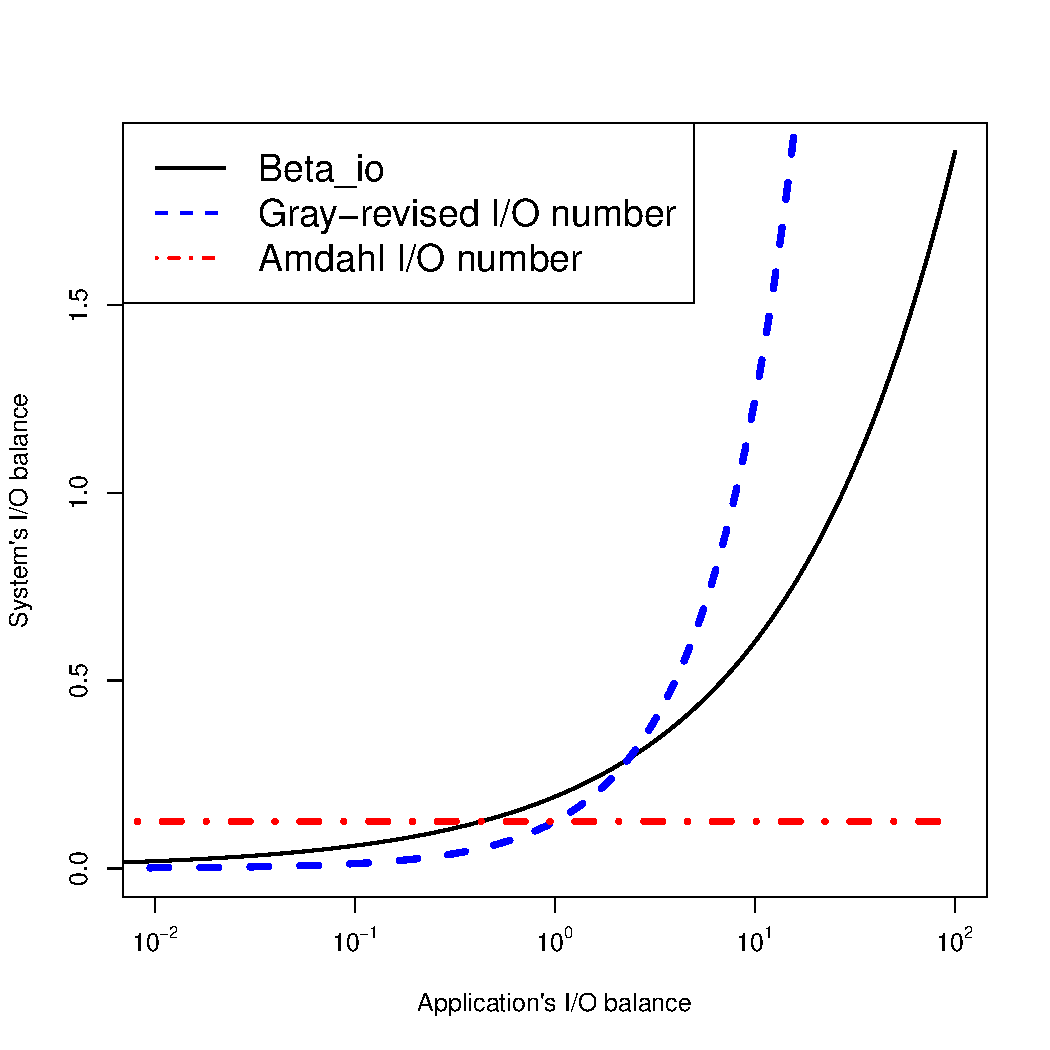
\includegraphics[width=\textwidth]{Figures/ModelFigures/beta_io.pdf}
                \caption{$\beta_{io}$ vs  $\gamma_{io}$}
                \label{fig:beta_io}
    \end{subfigure}
 	\begin{subfigure}[b]{0.48\textwidth}
                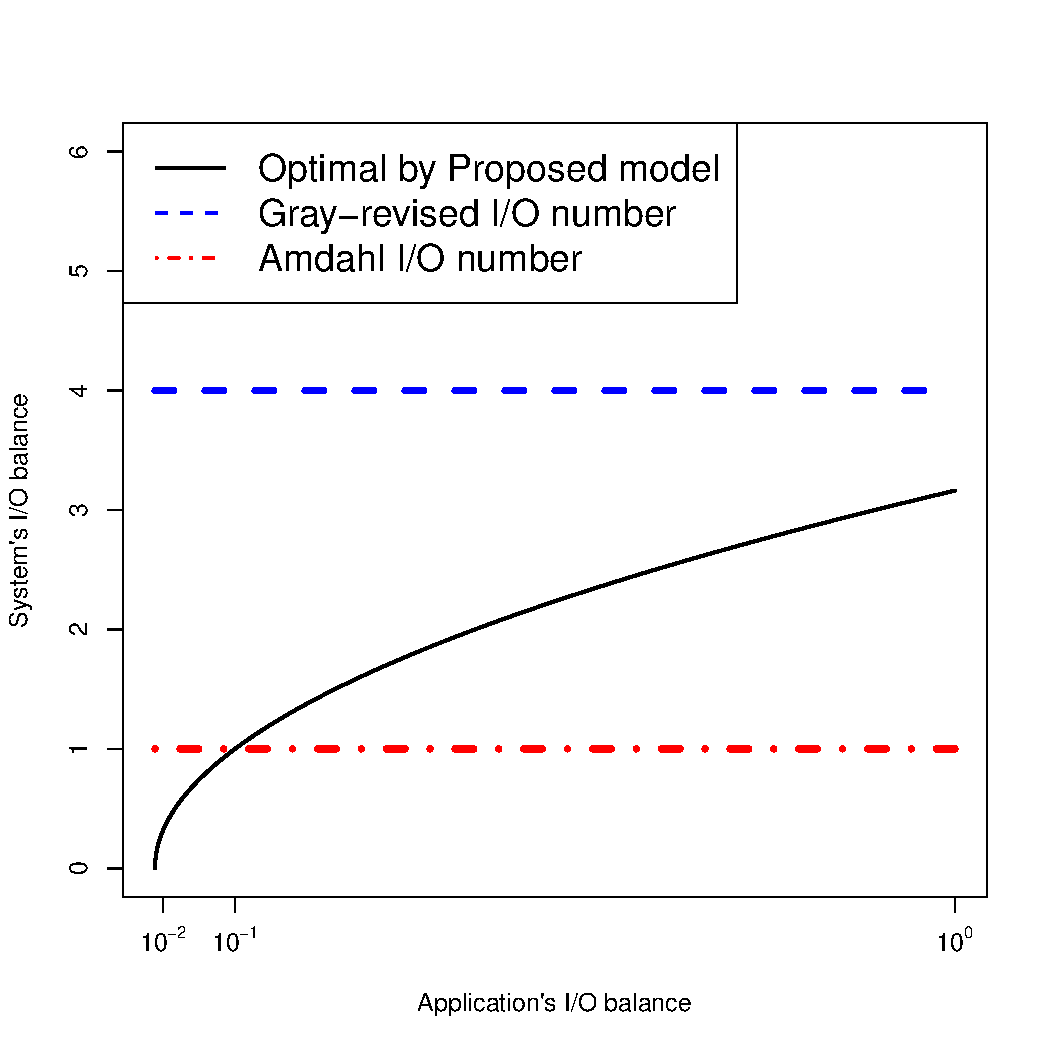
\includegraphics[width=\textwidth]{Figures/ModelFigures/beta_mem.pdf}
                \caption{$\beta_{mem}$ vs  $\gamma_{mem}$}
                \label{fig:beta_mem}
   \end{subfigure}
   \caption{Change in system's optimum I/O and memory balance ($\beta_{io}$ and $\beta_{mem}$) with respect to Intel Xeon processor ($\delta_{io} = 13.57$ and $\delta_{mem} = 0.08$) for different types of applications (varying values of $\gamma_{io}$ and $\gamma_{mem}$)}
  \label{fig:BetaVsGamma}
\end{figure*}
Figure-\ref{fig:beta_io} and \ref{fig:beta_mem} shows the change in system's optimum I/O and memory balance respectively with respect to Intel Xeon processor architecture for varying application balance (i.e., application's resource requirement). Based upon this figure characterize each of our experimental testbeds on the basis of $\beta_{io}$ and $\beta_{mem}$ and discuss the major pros and cons of each different architecture.  

%In this section we characterize each cluster on the basis of system balance parameters that we derived earlier and discuss the major pros and cons of each different cluster architecture. Since all the clusters in our evaluation use the same processor family (i.e., Intel Xeon) we use Equation-?? and ?? to calculate the Amdahl’s I/O and memory numbers of different clusters.
\subsubsection{SuperMikeII (Traditional HPC cluster)}
SuperMikeII has two 8-core Intel Sandybridge Xeon processor per node thus offering huge processing power. However, each SuperMikeII node is equipped with only one HDD, thus, limited in terms of I/O bandwidth. Also, each SuperMikeII node has only 32GB DRAM. Thus, SuperMikeII has both, $\beta_{io}=0.003$ and $\beta_{mem}=0.77$ a magnitude smalller than the optimum produced by our model for a data-, compute- and memory-intensive application as shown in Equation-\ref{eqn:BalancedOptIo} and Equation-\ref{eqn:BalancedOptMem}. According to Figure-\ref{fig:BetaVsGamma} SuperMikeII can provide optimal performance only for compute-intensive applications, precisely for those application with $\gamma_{io}=x$ and $\gamma_{mem}=y$.  
\subsubsection{SwatIII (Existing Datacenter)}
Unlike SuperMikeII which use only one HDD per node, SwatIII uses 4-HDDs per node using JBOD (Just a Bunch of Disk) configuration while using the same processor (i.e. two 8-core Intel SandyBridge Xeon) as SuperMikeII. Since the I/O throughput increases linearly with number of disks, SwatIII's $\beta_{io}=0.015$ is higher than SuperMikeII but lower than the optimum produced by our model for an I/O- and compute-intensive application (Equation-\ref{eqn:BalancedOptIo}). On the other hand, each SwatIII node has 256GB DRAM, thus achieve very high value for $\beta_{mem}=6.15$. It is to be noticed that $\beta_{mem}$ of SwatIII is even higher than the optimum produced by the model (Equation-\ref{eqn:BalancedOptMem}). Thus, according to Figure-\ref{fig:BetaVsGamma} SwatIII can produce optimal performance for moderately I/O-intensive applications and for memory-intensive applications, precisely when $\gamma_{io} = x$ and $\gamma_{mem}=y$.
\subsubsection{CeresII (MicroBrick-based Hyperscale System)}
The last one, CeresII is a novel hyperscale system based on Samsung MicroBricks. It uses one 6-core Intel Xeon processor with a core frequency of 2-GHz. Each MicroBrick (or,simply the computation module) of CeresII consists of a 6-core Intel Xeon processor with a core frequency of 2-GHz, two NVMe-SSD (Samsung) each with an I/O bandwidth of 2GBPS, and 64-GB DRAM. $\beta
_{io}$ of CeresII is $0.32$ which is closer to the optimum produced by our model in Equation-\ref{eqn:BalancedOptIo}.  On the other hand, $\beta_{mem}$ of each CeresII module is $5.33$. Although, it is higher than the optimal, it is significantly less than SwatIII. Thus, CeresII is the most balanced cluster among all the avalilable resources and we expect to get the best cost to performance for today's I/O-, compute- and memory-intensive applications for which  $\gamma_{io} = \gamma_{mem} = 1$. 

\section{Cluster Evaluation Methodology} \label{sec:EvalMethod}
To evaluate the clusters shown in Table-\ref{tab:Testbeds}, we use SuperMikeII as the baseline cofiguration and compare the performance of other clusters with respect to this. We always use homogeneous configuration across any cluster. One of the nodes in each cluster configuration is always used as Hadoop MasterNode. All other nodes are used as DataNodes.

\subsection{Software platform: Hadoop and Giraph}
To evaluate the relative merits of the clusters with respect to data-intensive scientific applications, first we need a big data analytic platform. The obvious selection is Hadoop which is nowadays the de facto standard for big data analysis and rapidly gaining popularity in scientific computing. We also evaluate the cluster hardware with respect to Giraph which is a large scale graph processing framework developed atop Hadoop. We use Clouera-Hadoop-2.3.0 and Giraph-1.1.0 for the entire study and use the Cloudera-Manager-5.0.0 for monitoring the system behavior. 

%Hadoop and Giraph were originated as the open-source counterpart of Google's MapReduce \cite{fw:mapreduce} and Pregel \cite{fw:pregel} respectively. Both the software read the input data from the underlying Hadoop Distributed File System (HDFS) in the form of disjoint sets or partitions of records. Then, in the MapReduce abstraction, a user-defined map function is applied to each disjoint set concurrently to extract information from each record in the form of intermediate key-value pairs. These key-value pairs are then grouped by the unique keys and shuffled to the reducers. Finally, a user-defined reduce function is applied to the value-set of each key, and the final output is written to the HDFS. The MapReduce framework enables data- and compute-intensive applications to run large volume of distributed data sets over distributed compute nodes with local storage. On the other hand, Giraph uses the Bulk Synchronous Parallel model \cite{fw:bsp} where computation proceeds in supersteps. In the first phase of a superstep, Giraph leverages Hadoop-mappers when a user-defined vertex-program is applied to all the vertices concurrently. In the end of each superstep, each vertex can send a message to other vertices to initiate the next superstep. Alternatively, each vertex can vote to halt. The computation stops when all the vertices vote to halt unanimously in the same superstep. Giraph enables memory- and compute-intensive applications to upload data into distributed memories over different compute nodes.

\subsection{Hadoop Configurations Overview}
Since our goal is to evaluate the underlying hardware components and their, we avoid any unnecessary change in the source code of Hadoop or Giraph. To evaluate the balance between the hardware components, we set up the Hadoop parameters such that the application can make use of the maximum available processing speed, I/O bandwidth and DRAM. However, it is worthy to mention here, due to limited I/O bandwidth in SuperMikeII (traditional HPC cluster with only 1-HDD per node) we could launched only 8 concurrent YARN containers (i.e., 8 concurrent map/reduce tasks) i.e.,half of the total number of cores to get the optimal performance. Appendix-\ref{app:HadoopConfigurationsAndoptimizations} shows a brief description of our Hadoop configurations.

\subsection{Benchmark Application Characteristics}
\begin{table*}
\caption{Data size for different benchmark applications}
\label{tab:AppChar}
\begin{center}
    \begin{tabular}{ |p{3cm} | p{1.5cm} | p{2.5cm} | p{2.5cm} | p{0.8cm} | p{0.8cm} | p{0.8cm} | p{2.5cm}|} \hline
     Job name & Job Type & Input & Final output & \# jobs & Shuffled data & HDFS Data & Application Characteristics \\ \hline
    Terasort & Hadoop & 1TB & 1TB & 1 & 1TB & 1TB & Map: CPU-intensive, Reduce: I/O-intensive \\ \hline
    Wordcount & Hadoop & 1TB & 1TB & 1 & 1TB & 950GB & Map and Reduce: CPU-Intensive \\ \hline 
   Graph Construction (moderate size bumble bee genome)  & Hadoop & 90GB (500-million reads) & 95GB & 2 & 2TB & 136GB & Map and Reduce: CPU- and I/O-intensive \\ \hline
    Graph Simplification (moderate size bumble bee genome) & Series of Giraph jobs & 95GB (71581898 vertices) & 640MB (62158 vertices) & 15 & - & 966GB & Memory-intensive\\ \hline    
    Graph Construction (large size human genome) & Hadoop & 452GB (2-billion reads) & 3TB & 2 & 9.9TB & 3.2TB &Map and Reduce: CPU- and I/O-intensive\\ \hline
    Graph Simplification (large size human genome) & Series of Giraph jobs & 3.2TB (1483246722 vertices) & 3.8GB (3032297 vertices) & 15 & - & 4.1TB & Memory-Intensive \\ \hline 
    \end{tabular}
\end{center}
\end{table*}
Table-\ref{tab:AppChar} summarizes the details of the benchmark applications, the data size handled by each of these applications and their corresponding characteristics. We used three benchmark application for our evaluation: TeraSort, WordCount, and a real world genome assembly application. A brief description of each of these applications are as follows:

\subsubsection{TeraSort}
The first one is TeraSort, a standard benchmark for any data processing framework. The Hadoop version of TeraSort samaples and partitions the input data in its map phase based upon only first few characters. The reduce phase then uses quicksort algorithm to sort each of the partition locally. 
The map phase of TeraSort is CPU-intensive as it reads only the first few characters of each row in the input dataset to generate the key (called sample-key) for each data. However, based upon the data size reduce phase can be severely I/O-intensive. The entire dataset needs to be transferred to different reducers and each reducer needs to read each row at least once to sort the data set. Again, for huge volume of data partition, that cannot fit in memory, an external sort may be applied making the reduce phase severely I/O intensive.  

\subsubsection{WordCount}
The second one is WordCount, another widely used Hadoop benchmark. The map phase of WordCount parse the input data set line by line to extract each word. Each word is emmitted with a $1$ as its initial count which is then summed up in the reduce phase to output its  freauency. 
Since both the map and reduce phase read the entire data set sequentially just once, both the map and reduce phase of WordCount is CPU-intensive. 

\subsubsection{Genome Assembly}
The third one is a genome assembly application that we developed based on Hadoop and Giraph to address the challenges in large scale genome assembly that recently made its way to the forefront of big data challenges. The first phase uses Hadoop to scan the genome data set to filter out the lines containing only neucleotide characters (i.e., $A$, $T$, $G$, and $C$) and then divides each of those lines into smaller fragments of length $k$ known as $k$-mer. Map phase emits each two subsequent $k$-mers as key-value pair representing a vertex and an edge from it. The reduce phase then aggregates all the edges emmitted from each vertex to write the entire graph structure to HDFS. The second phase of the assembly application uses Giraph to to compress each of the linear chains in the graph structure to one vertex and remove the tip and bubble structure in the graph (included because of sequencing error). After removing the tips and bubble structure the graph may have some new linear chains which are compresed again. Similarly, new tip and bubble structures are removed again. So, the process continues incrementally as a series of Giraph jobs until there is no tip or bubble in the graph. Appendix-\ref{app:GenomeAssemblyAlgorithms} shows the overview of the algorithms used in our genome assembly application.

\subsection{Data Size}
For both TeraSort and WordCount benchmark, we ran TeraGen program and generated another 1TB random dataset as the input for these benchmark. Both TeraSort and WordCount generate almost similar amount data in the intermediate shuffle phase as their input. The output data size of TeraSort is also same as its input (i.e., 1TB in this work) whereas, the output of WordCount may vary based upon the frequency of different words in the randomly generated dataset. In our case it was almost 950GB.

For the genome assembly benchmark application, in this work we use two different genome datasets: 1) a moderate size bumble bee genome dataset (90GB) and 2) a large size human genome dataset (452GB). The corresponding graph sizes are 95GB and 3.2TB based upon the number of unique $k$-mers (using $k=31$ in both the cases) in the data set. The Hadoop stage of the assembly application is severely shuffle intensive. For both the dataset the size of the temporary shuffle data isalmost 21-times more than the input size. The bumble bee genome is available in Genome Assembly Gold-standard Evaluation (GAGE \cite{bio:gage}) website\footnote{http://gage.cbcb.umd.edu/} in fastq format. The Human genome is available in NCBI website with accession number SRX016231\footnote{http://www.ncbi.nlm.nih.gov/sra/SRX016231[accn]}.

\section{Result and Discussion} \label{sec:Result}
\subsection{Evaluating the Cost/Performance of Different Cluster with TeraSort, WordCount and Bumble bee genome assembly}
\begin{table}[!t]
\caption{Resources available for each cluster architecture keeping the total cost of the cluster same. The cost of 15 datanodes of SuperMikeII is used as baseline}
\label{tab:ScalingCost}
\label{fig:perf}
\centering
\begin{tabular}{|p{2.5cm}|p{1.5cm}|p{1.5cm}|p{1.5cm}|p{1.5cm}|} \hline
Cluster Configurations & SuperMikeII & SwatIII & CeresII\\ \hline
Total cost (\$) & 57060 & 57060 & 57060\\ \hline
Cost/DN (\$) & 3804 & 6911 & 2282\\ \hline
\#DN & 15 & 8 & 25\\ \hline
Total processing speed (GHz) & 624.00 & 330.83 & 300.00\\ \hline
Total I/O bandwidth (GBPS) & 2.25 & 4.80 & 50.00\\ \hline
Total storage space (TB) & 7.50 & 16.00 & 25.00\\ \hline
Total DRAM Size (TB) & 0.48 & 2.00 & 1.60\\ \hline
\end{tabular}
\end{table}
\begin{figure}[!t]
\centering
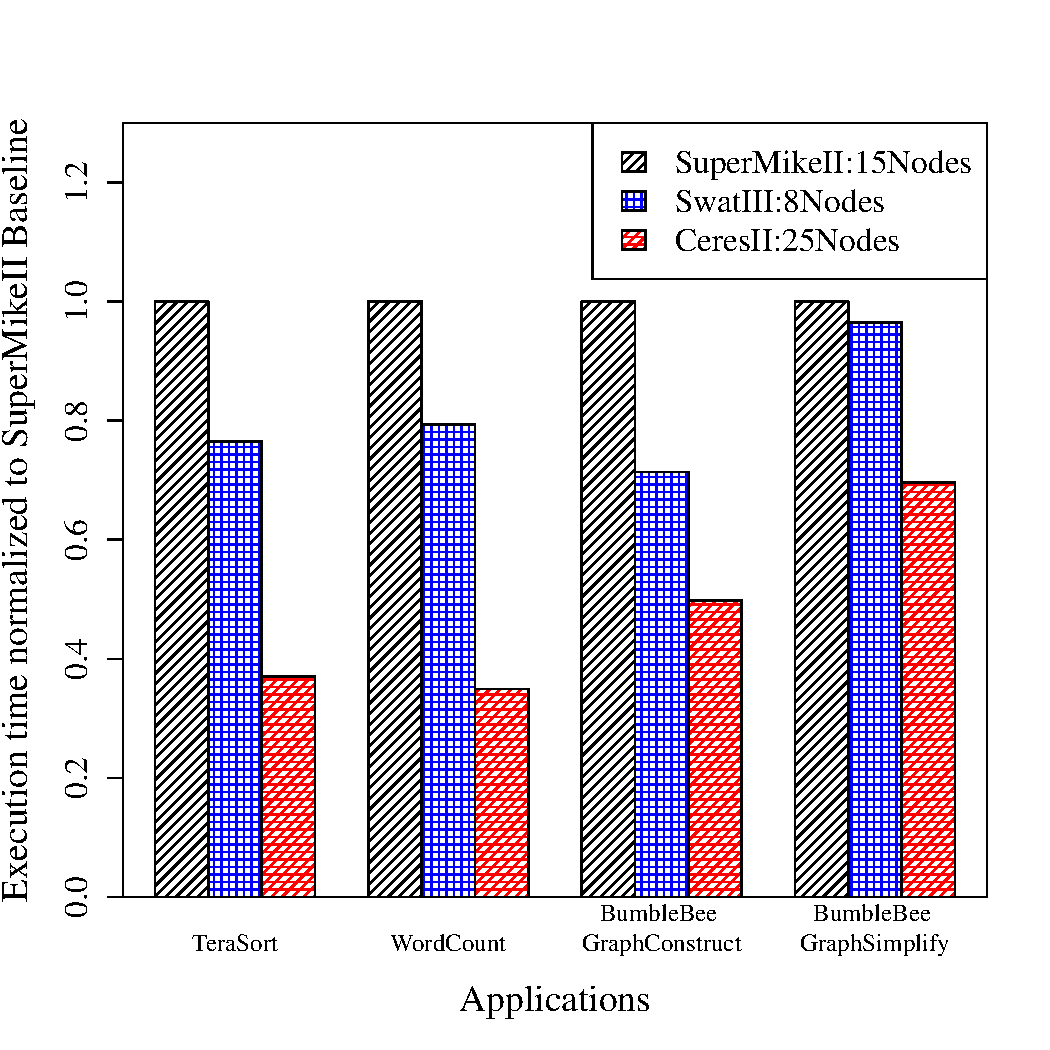
\includegraphics[width=.5\textwidth]{Figures/PerformanceFigures/execTime.pdf}
\caption{Performance of different cluster architecture for different applications keeping the total cost of each cluster same}
\end{figure}
To show the balance between performance and economy we keep the total cost same across all the clusters. Table-\ref{tab:Cost} shows the available resources for all the three cluster architectures available to us i.e. SuperMikeII, SwatIII and CeresII while keeping the total cost same across all the clusters. We used the cost of $15$ datanodes of SuperMikeII as the baseline. Then, we divided this baseline-cost by the cost of each node in SwatIII and CeresII to count the number of nodes to be used in these two different clusters.

We ran the first three applications described in Table-\ref{tab:AppChar} in all the three cluster configurations and measured their execution time. All results are the means of at least 3 runs of each job on each configuration. Figure-\ref{fig:perf} shows the results normalized to the SuperMikeII baseline. That is, the  execution time of SuperMikeII is always $1$. We see that CeresII being closer to the optimal produced by our model performs surprisingly well: 
\begin{enumerate}
\item Comparing to SuperMikeII baseline, for both TeraSort and WordCount benchmark application, CeresII shows almost 65\% improvement. For Hadoop and Giraph stage of the bumble bee (90GB) genome assembly application, it shows almost 50\%  and 30\% improvement respectively over the baseline. 
\item Comparing to SwatIII, CeresII shows almost 50\% improvement in execution time for TeraSort and WordCount. For the our genome assembly benchmark evaluation it CeresII shows almost 30\% improvement in tboth he Hadoop and Giraph stage of assembly respectively. 
\end{enumerate}

\subsection{System Characteristics}
\begin{figure*}[htb]
	\begin{subfigure}[b]{0.24\textwidth}
                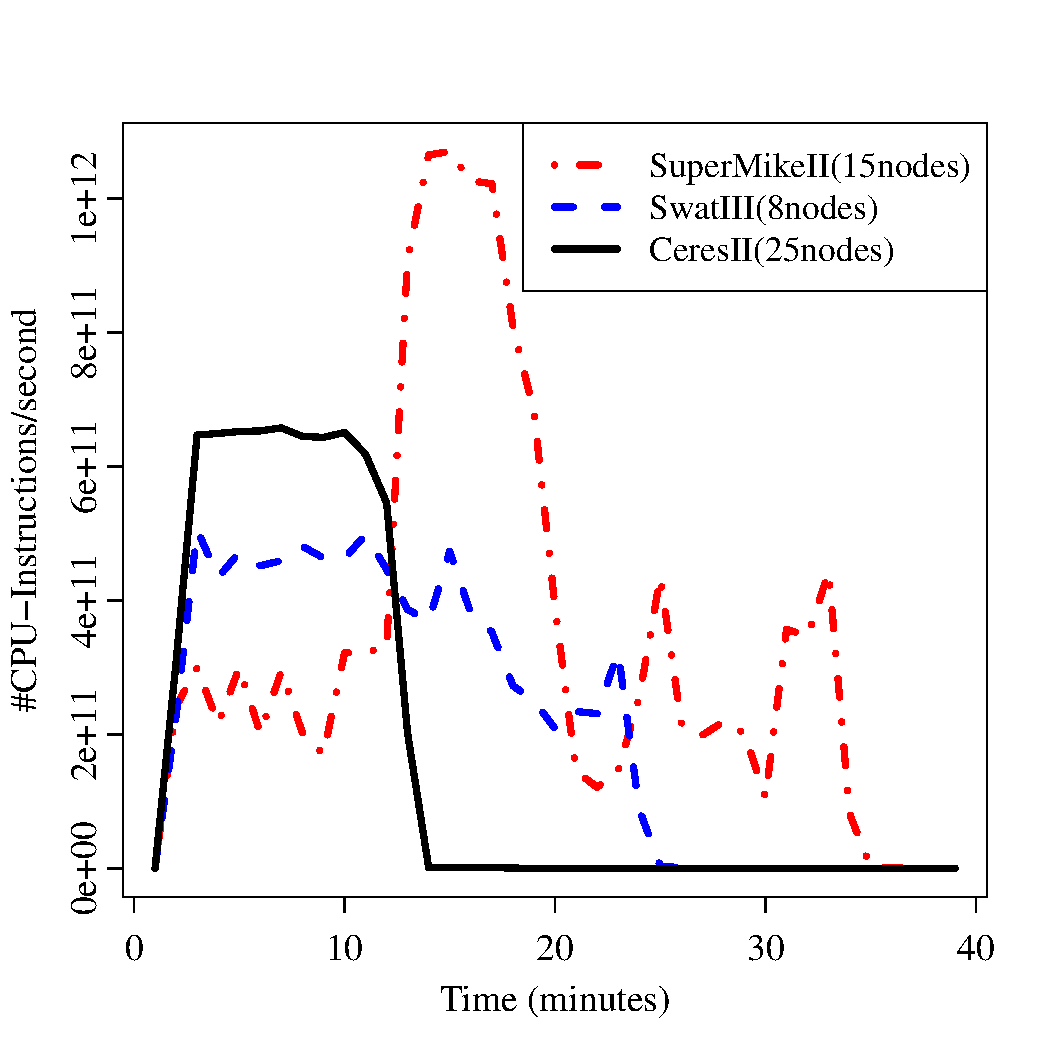
\includegraphics[width=\textwidth]{Figures/SystemFigures/TeraSortIPS.pdf}
                \caption{TeraSort}
                \label{fig:TeraSortIPS}
    \end{subfigure}
 	\begin{subfigure}[b]{0.24\textwidth}
                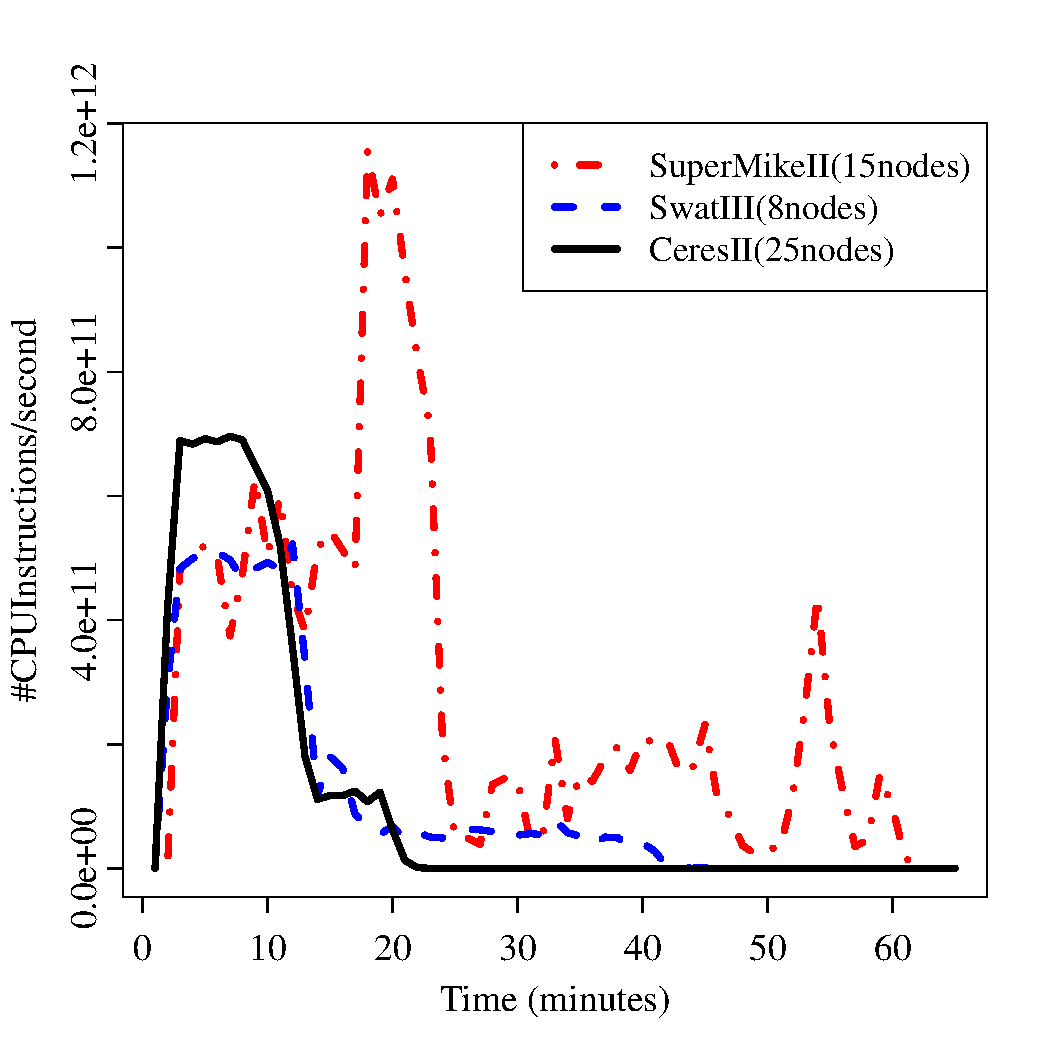
\includegraphics[width=\textwidth]{Figures/SystemFigures/WordCountIPS.pdf}
                \caption{WordCount}
                \label{fig:WordCountIPS}
   \end{subfigure}
   \begin{subfigure}[b]{0.24\textwidth}
                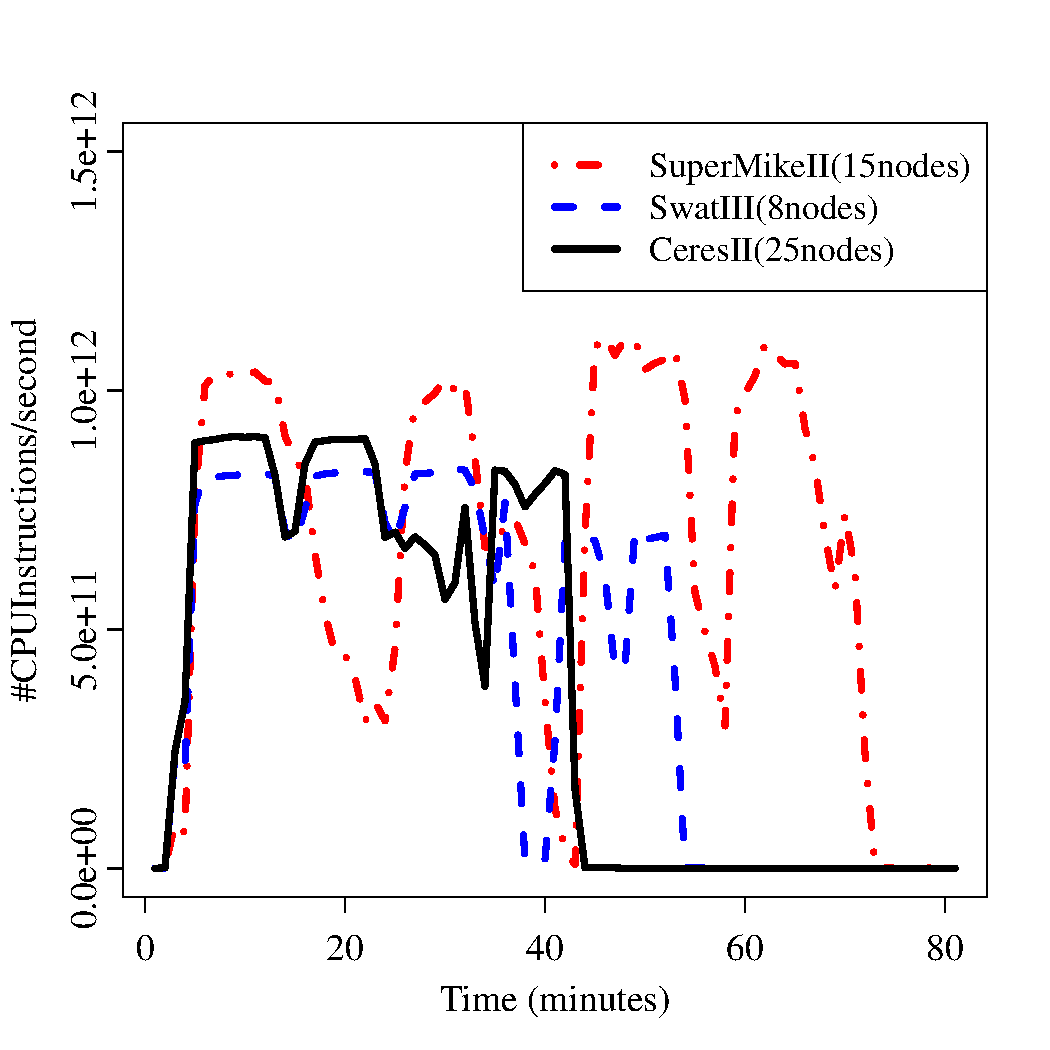
\includegraphics[width=\textwidth]{Figures/SystemFigures/BombusGrConsIPS.pdf}
                \caption{Bumble bee Hadoop}
                \label{fig:BombusGrConsIPS}
    \end{subfigure}
 	\begin{subfigure}[b]{0.24\textwidth}
                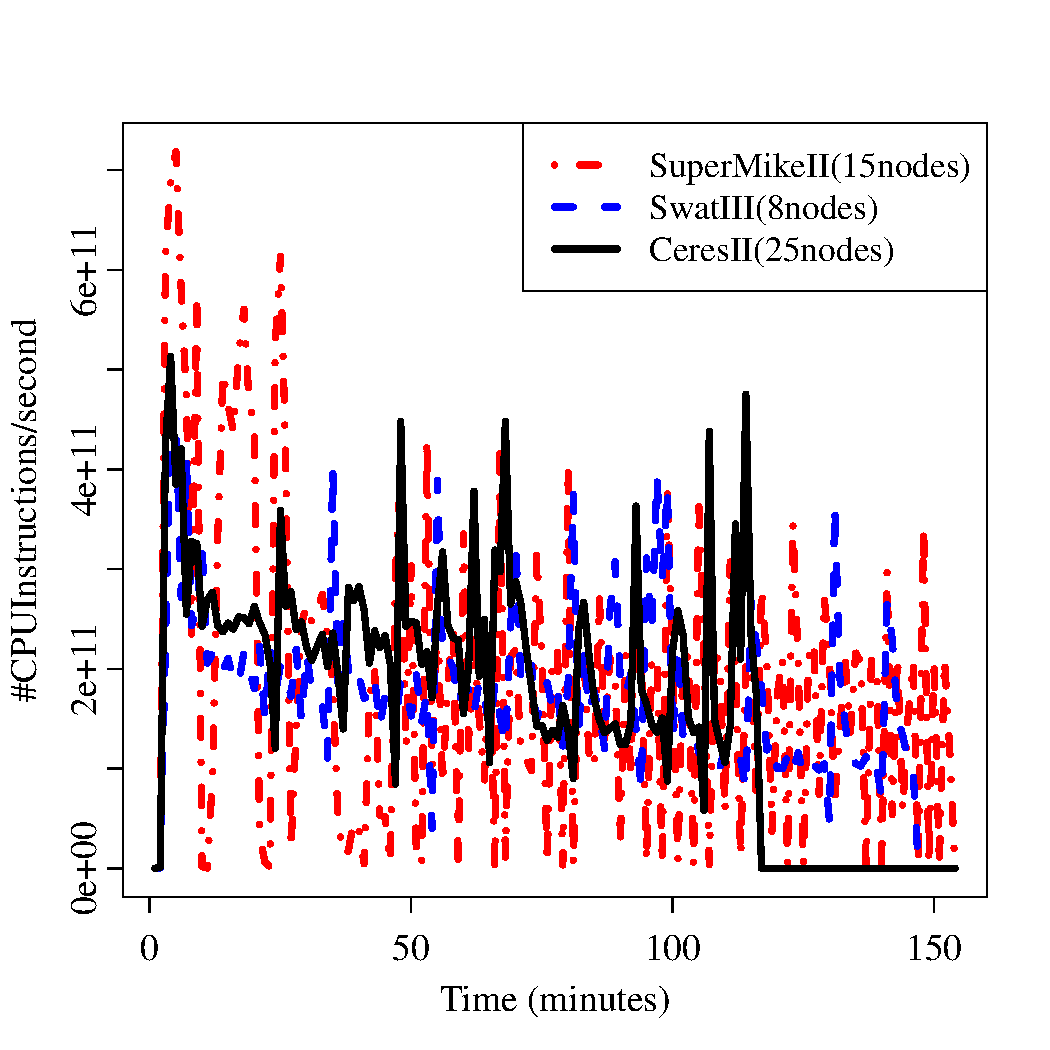
\includegraphics[width=\textwidth]{Figures/SystemFigures/BombusGrSimpIPS.pdf}
                \caption{BumbleBee Giraph}
                \label{fig:BombusGrSimpIPS}
   \end{subfigure}
   \caption{Instruction per second}
  \label{fig:IPS}
\end{figure*}
\begin{figure*}[htb]
	\begin{subfigure}[b]{0.24\textwidth}
                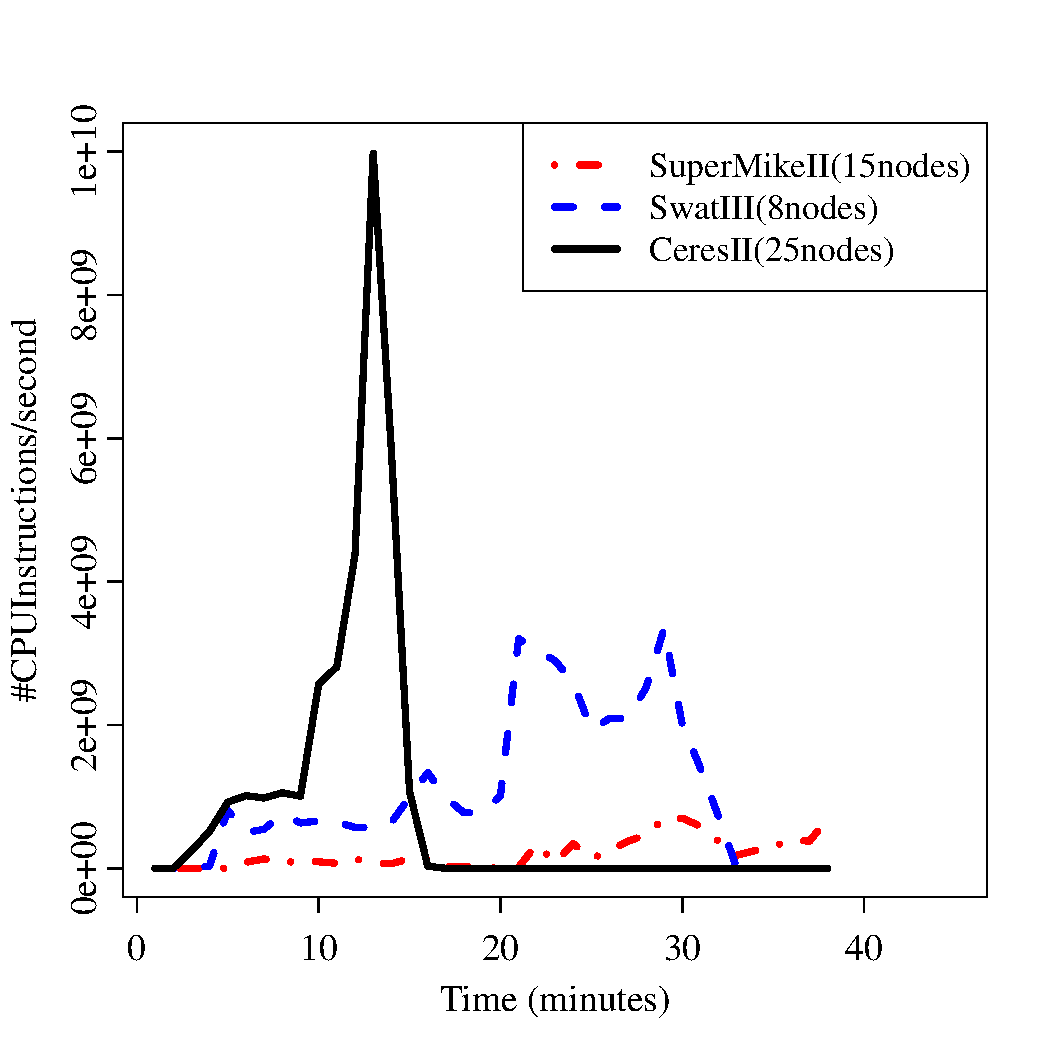
\includegraphics[width=\textwidth]{Figures/SystemFigures/TeraSortIO.pdf}
                \caption{TeraSort}
                \label{fig:TeraSortIO}
    \end{subfigure}
 	\begin{subfigure}[b]{0.24\textwidth}
                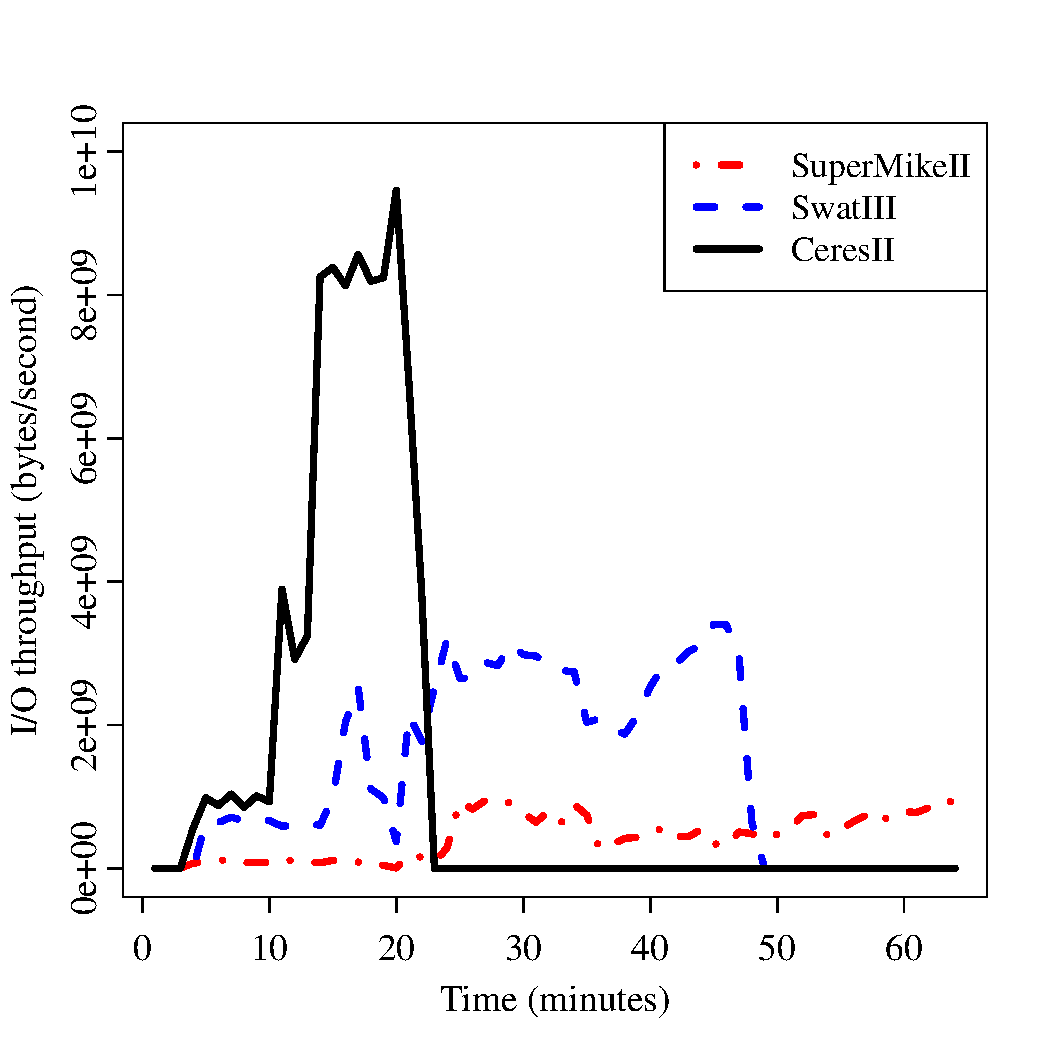
\includegraphics[width=\textwidth]{Figures/SystemFigures/WordCountIO.pdf}
                \caption{WordCount}
                \label{fig:WordCountIO}
   \end{subfigure}
   \begin{subfigure}[b]{0.24\textwidth}
                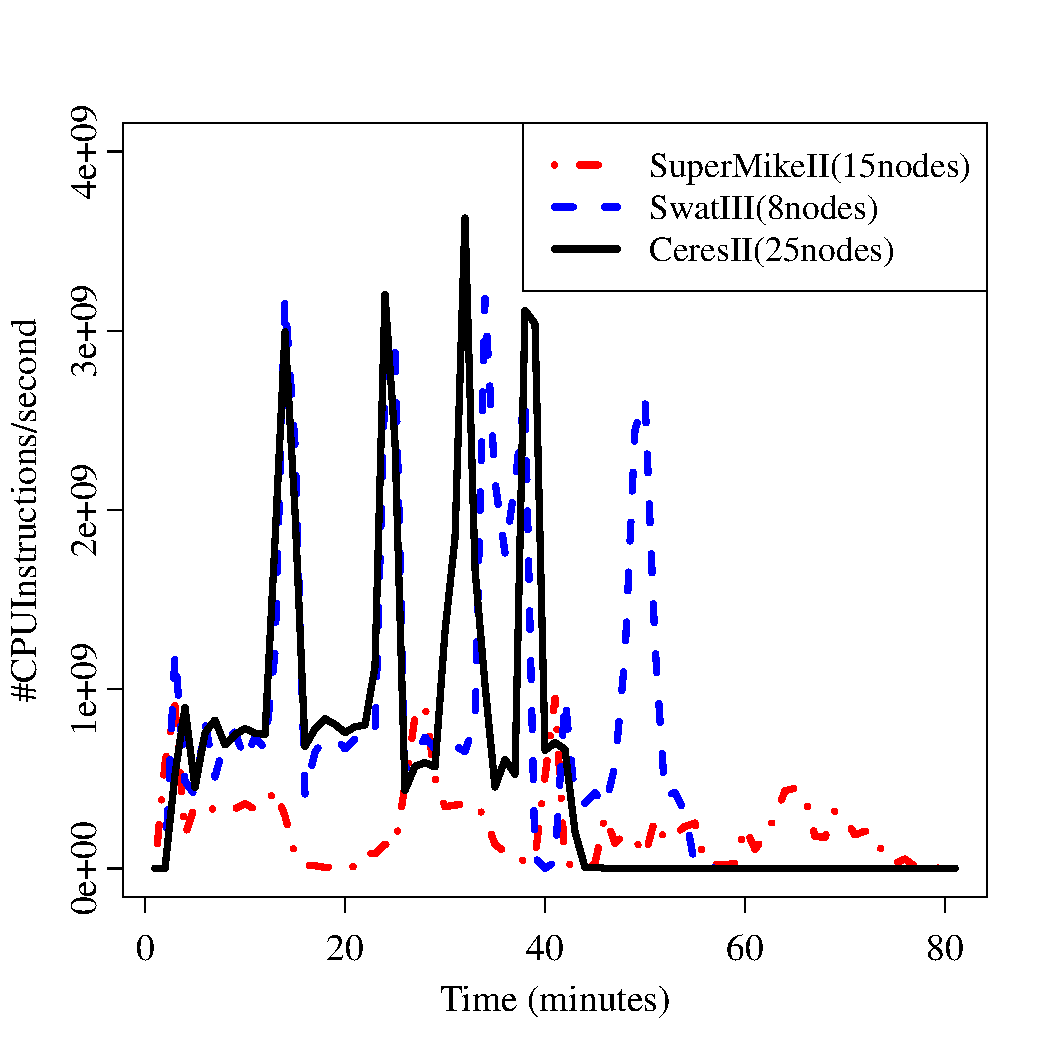
\includegraphics[width=\textwidth]{Figures/SystemFigures/BombusGrConsIO.pdf}
                \caption{Bumble bee Hadoop}
                \label{fig:BombusGrConsIO}
    \end{subfigure}
 	\begin{subfigure}[b]{0.24\textwidth}
                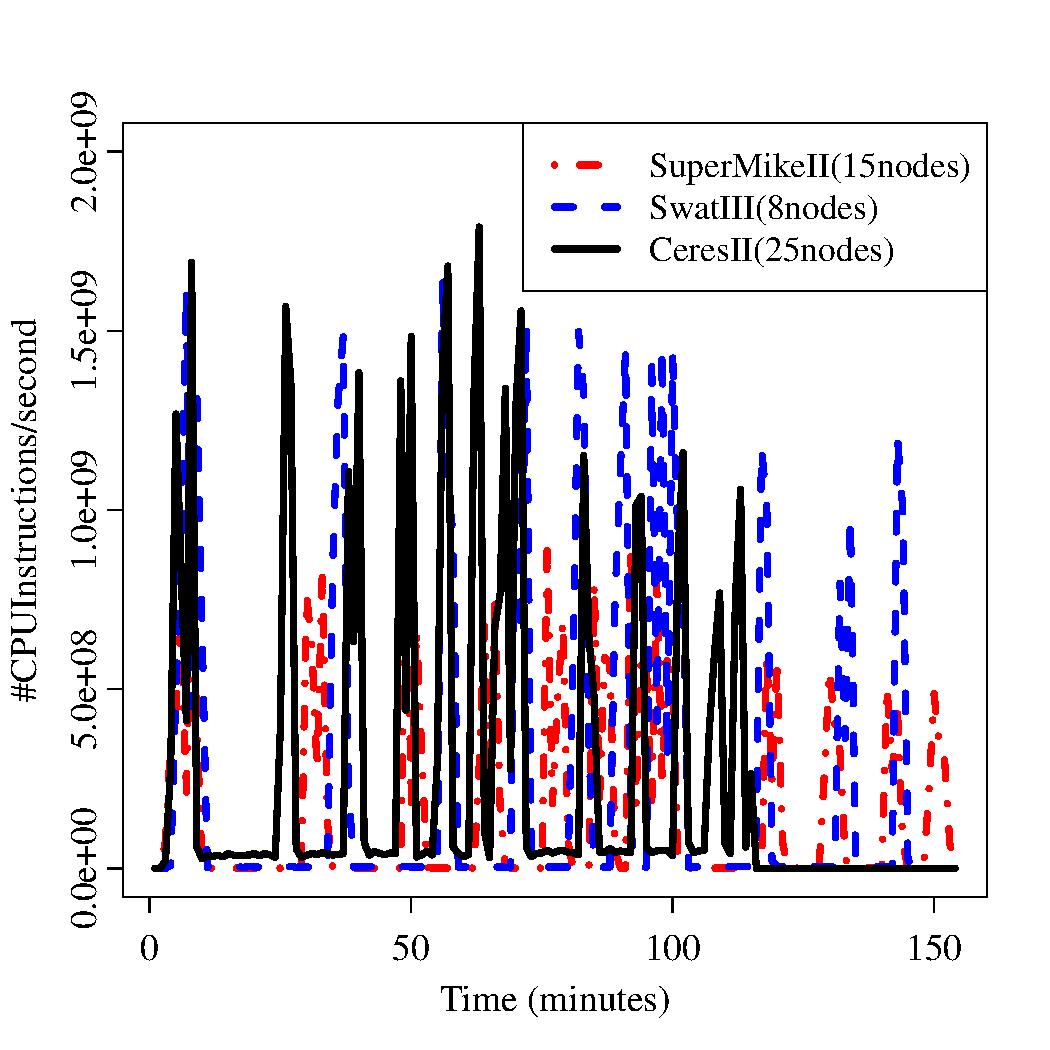
\includegraphics[width=\textwidth]{Figures/SystemFigures/BombusGrSimpIO.pdf}
                \caption{BumbleBee Giraph}
                \label{fig:BombusGrSimpIO}
   \end{subfigure}
   \caption{I/O Bandwidth}
  \label{fig:IO}
\end{figure*}
Figure-\ref{fig:IPS} and \ref{fig:IO} shows the total number of CPU instructions per second (IPS) and I/O bandwith acorss different cluster architecture while keeping the total cost of the cluster same. For both TeraSort and WordCount, the peak IPS of SuperMikeII is significantly higher than both SwatIII and CeresII. However, the average I/O bandwidth of SuperMikeII is significantly less than the other two leading to significantly high I/O wait which resulting in lower average IPS. This huge difference between peak and average IPS is because of the extremely low value of $\beta_{io}$ in SuperMikeII.

SwatIII cluster shows a better balance between CPU and I/O than SuperMikeII. However, because of its high size of DRAM, it gives up processing speed with respect to CeresII (128 core in SwatIII vs 150 cores in CeresII) when the total cost of the cluster is same. 

CeresII cluster is the optimally balnced in terms of CPU speed and I/O bandwidth with a $\beta_{io}$ value of 0.19. Figure-\ref{fig:TeraSortIPS} and \ref{fig:WordCountIPS} shows that CeresII achieves higher Peak IPS than SwatIII but less than SuperMikeII for both TeraSort and WordCount application. On the other hand, CeresII achieves significantly higher I/O bandwidth than both the cluster keeping the peak and average IPS of the application almost similar and finally leading to the lowest execution time for any of the applications.

\subsection{Evaluating Different Cluster for Large Size Human Genome Assembly}
\begin{table}[!t]
\caption{Maximum available resources in each cluster architecture}
\label{tab:TotalCluster}
\label{fig:perf}
\centering
\begin{tabular}{|p{2.5cm}|p{1.5cm}|p{1.5cm}|p{1.5cm}|p{1.5cm}|} \hline
Cluster Configurations & SuperMikeII & SwatIII & CeresII\\ \hline
Total cost (\$) & 486912 & 110576 & 91280\\ \hline
Cost/DN (\$) & 3804 & 6911 & 2282\\ \hline
\#DN & 128 & 16 & 40\\ \hline
Total processing speed (GHz) & 5324.8 & 665.6 & 480.00\\ \hline
Total I/O bandwidth (GBPS) & 19.2 & 9.60 & 80.00\\ \hline
Total storage space (TB) & 7.50 & 16.00 & 25.00\\ \hline
Total DRAM Size (TB) & 4 & 4 & 2.5\\ \hline
\end{tabular}
\end{table}
\begin{figure}[htb]
	\begin{subfigure}[b]{0.23\textwidth}
                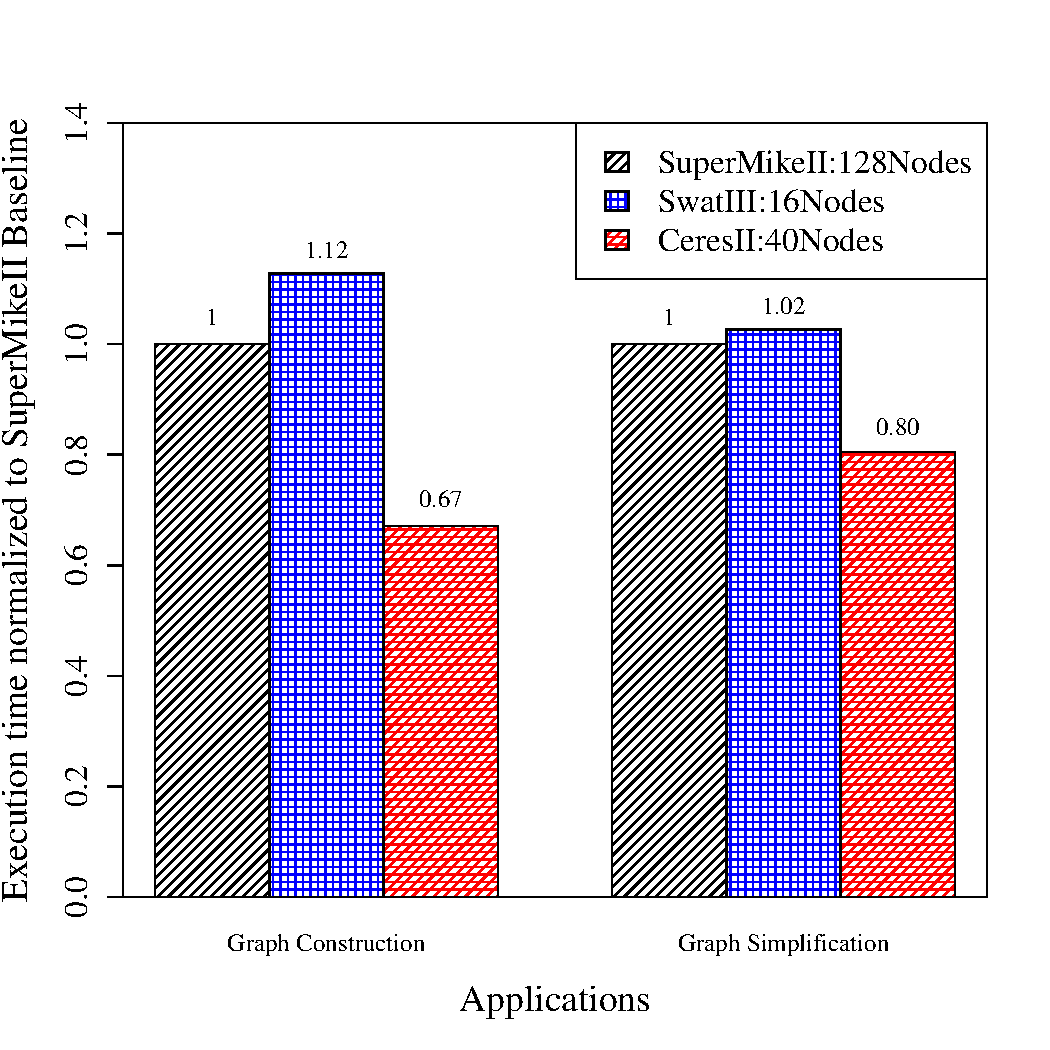
\includegraphics[width=\textwidth]{Figures/PerformanceFigures/execTimeHum.pdf}
                \caption{$\beta_{io}$ vs  $\gamma_{io}$}
                \label{fig:HumPerf}
    \end{subfigure}
 	\begin{subfigure}[b]{0.23\textwidth}
                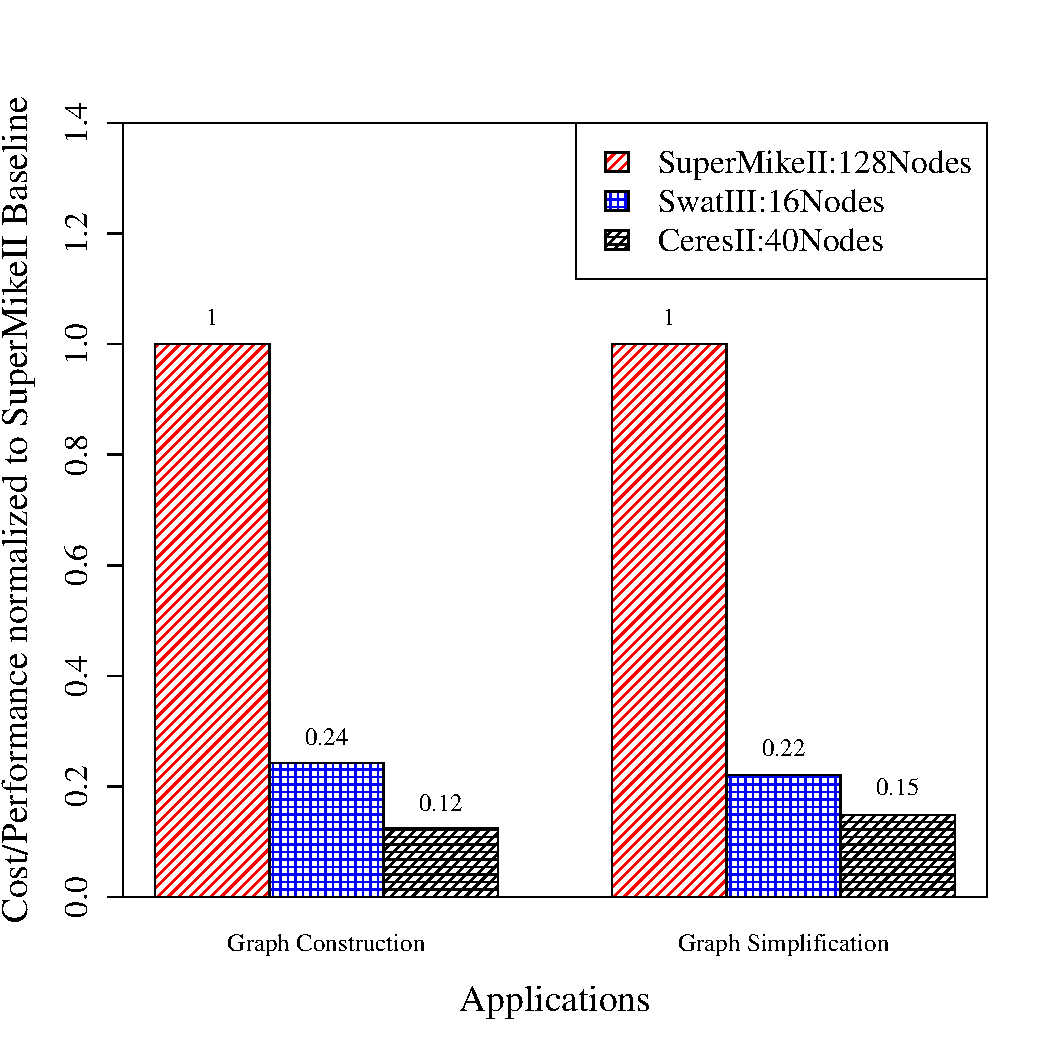
\includegraphics[width=\textwidth]{Figures/PerformanceFigures/costTimeHum.pdf}
                \caption{$\beta_{mem}$ vs  $\gamma_{mem}$}
                \label{fig:HumCost}
   \end{subfigure}
   \caption{Performance of different cluster for large size human genome assembly}
  \label{fig:Hum}
\end{figure}
to assemble the large human genome (452GB) we used the maximum available resources in each of the clusters to accommodate the huge amount of shuffled data (9.9TB) as well as the graph data (3.2TB). That is, we used all 128 nodes of SuperMikeII, 16 nodes of SwatIII, and 40 nodes of CeresII for this application. Figure-\ref{fig:HumPerf} and \ref{fig:HumCost} shows the execution time and the cost/performance respectively for the Hadoop and Giraph stage of the human genome assembly pipeline. As shown in the model, we consider the performance as the inverse of the execution time and multiplied the execution time with the total cost of each cluster to get the corresponding cost/performance. All data is again normalized to SuperMikeII baseline. The results are as follows:
\begin{enumerate}
\item CeresII even with only 9\% processing speed than SuperMikeII across the cluster, outperforms SuperMikeII by more than 30\% in the Hadoop stage of the assembly. In the Giraph stage, the performance gain is almost 20\%. In terms of cost/performance, the corresponding gains are 88\% and 85\% respectively. 
\item Comparing to SwatIII,  the processing power of CeresII is 72\%. However,  due to the optimal architectural balance, CeresII outperforms SwatIII by almost 50\% in the Hadoop stage. The corresponding improvement in Giraph stage is 20\%. In terms of cost/performance, CeresII shows almost 50\% and 30\% improvement over SwatIII for Hadoop and Giraph stage respectively.
\end{enumerate}

% An example of a floating figure using the graphicx package.
% Note that \label must occur AFTER (or within) \caption.
% For figures, \caption should occur after the \includegraphics.
% Note that IEEEtran v1.7 and later has special internal code that
% is designed to preserve the operation of \label within \caption
% even when the captionsoff option is in effect. However, because
% of issues like this, it may be the safest practice to put all your
% \label just after \caption rather than within \caption{}.
%
% Reminder: the "draftcls" or "draftclsnofoot", not "draft", class
% option should be used if it is desired that the figures are to be
% displayed while in draft mode.
%
%\begin{figure}[!t]
%\centering
%\includegraphics[width=2.5in]{myfigure}
% where an .eps filename suffix will be assumed under latex, 
% and a .pdf suffix will be assumed for pdflatex; or what has been declared
% via \DeclareGraphicsExtensions.
%\caption{Simulation results for the network.}
%\label{fig_sim}
%\end{figure}

% Note that the IEEE typically puts floats only at the top, even when this
% results in a large percentage of a column being occupied by floats.


% An example of a double column floating figure using two subfigures.
% (The subfig.sty package must be loaded for this to work.)
% The subfigure \label commands are set within each subfloat command,
% and the \label for the overall figure must come after \caption.
% \hfil is used as a separator to get equal spacing.
% Watch out that the combined width of all the subfigures on a 
% line do not exceed the text width or a line break will occur.
%
%\begin{figure*}[!t]
%\centering
%\subfloat[Case I]{\includegraphics[width=2.5in]{box}%
%\label{fig_first_case}}
%\hfil
%\subfloat[Case II]{\includegraphics[width=2.5in]{box}%
%\label{fig_second_case}}
%\caption{Simulation results for the network.}
%\label{fig_sim}
%\end{figure*}
%
% Note that often IEEE papers with subfigures do not employ subfigure
% captions (using the optional argument to \subfloat[]), but instead will
% reference/describe all of them (a), (b), etc., within the main caption.
% Be aware that for subfig.sty to generate the (a), (b), etc., subfigure
% labels, the optional argument to \subfloat must be present. If a
% subcaption is not desired, just leave its contents blank,
% e.g., \subfloat[].


% An example of a floating table. Note that, for IEEE style tables, the
% \caption command should come BEFORE the table and, given that table
% captions serve much like titles, are usually capitalized except for words
% such as a, an, and, as, at, but, by, for, in, nor, of, on, or, the, to
% and up, which are usually not capitalized unless they are the first or
% last word of the caption. Table text will default to \footnotesize as
% the IEEE normally uses this smaller font for tables.
% The \label must come after \caption as always.
%
%\begin{table}[!t]
%% increase table row spacing, adjust to taste
%\renewcommand{\arraystretch}{1.3}
% if using array.sty, it might be a good idea to tweak the value of
% \extrarowheight as needed to properly center the text within the cells
%\caption{An Example of a Table}
%\label{table_example}
%\centering
%% Some packages, such as MDW tools, offer better commands for making tables
%% than the plain LaTeX2e tabular which is used here.
%\begin{tabular}{|c||c|}
%\hline
%One & Two\\
%\hline
%Three & Four\\
%\hline
%\end{tabular}
%\end{table}


% Note that the IEEE does not put floats in the very first column
% - or typically anywhere on the first page for that matter. Also,
% in-text middle ("here") positioning is typically not used, but it
% is allowed and encouraged for Computer Society conferences (but
% not Computer Society journals). Most IEEE journals/conferences use
% top floats exclusively. 
% Note that, LaTeX2e, unlike IEEE journals/conferences, places
% footnotes above bottom floats. This can be corrected via the
% \fnbelowfloat command of the stfloats package.




\section{Conclusion} \label{sec:Conclusion}
The conclusion goes here.




\appendices
\section{Hadoop Configuration and Optimization}
 \label{app:HadoopConfigurationsAndoptimizations}
The Hadoop configurations are similar to our previous work \cite{}. A brief description of the Hadoop-parameters that we changed are as follows:
  
\textbf{Number of concurrent YARN containers:} After performing rigorous testing,  we observed, that for SuperMikeII and SwatIII-Basic-HDD (1-HDD/DN cases), 8-conainers/DN (i.e., half of total cores/node) show the best result. For any other cluster, number of concurrent containers per datanode is kept equal to the number of cores per node. 

\textbf{Amount of memory per container and Java-heap-space:} In each node in any node of any cluster, we kept 10\% of the memory for the system use. The rest of the memory is equally divided among the launched containers. The Java heap space per worker is always set to lower than memory per container as per normal recommendation.

\textbf{Total number of Reducers:} Based on the observation of job profiles, we observed that 2-times of reducers than number of concurrent containers produce good performance in general. 

\textbf{Giraph workers:} The number of Giraph workers is set according to the number of concurrent YARN containers.

\textbf{Other Giraph parameters:} We always used enough memory to accommodate the graph structure in memory and always avoided using the out-of-core execution feature of Giraph, which writes huge data to the disk. We also avoided using the checkpoint feature for the same reason.


\section{Genome Assembly Algorithms}
\label{app:GenomeAssemblyAlgorithms}
%\subsubsection{TeraSort}
%TeraSort smaples the input data and uses MapReduce to sort the entire data. The map phase of TeraSort samples and partitions the entire dataset by reading only the first few characters of each row. Then, it assigns a key (called sample-key) to each partition of the input dataset. The sample-keys are generated such that, the sample-key of a partition (say $partition_i$) is less than the sample-key of the next partition (i.e., $partition_{i+1}$). Then,based upon these sample keys the data set is distributed over the reducers. Then each reducer uses quicksort to sort the local partitions of the data assigned to it. and the sorted data is written to the HDFS. 
%\subsubsection{WordCount}
%Hadoop WordCount is a workload that reads an input text file and counts how often a certain word exists in the text file. each line is fed into a mapper as an input and breaks down each line into words. It then uses a key/value pair for each word with $1$ next to each word as initial count. A reducer sums the count of each word and issues a key/value pair with the word and sum for each word and the final output is written to HDFS. 
The motivation behind selecting genome assembly application is that, the high throughput next generation DNA sequencing machines (e.g., Illumina Genome Analyzer) has outpased Moore's law and started producing a huge amount of short read sequences typically in the scale of several Gigabytes to Terabytes. Furthermore, the size of the de Bruijn graph built from these vast amount of short reads may be a magnitude higher than the reads itself making the entire assembly pipe line severely data-intensive.

De novo genome assembly refers to the construction of an entire genome sequence from a huge amount of small, overlapping and erroneous fragments called short read sequences while no reference genome is available. The problem can be mapped as a simplified de Bruijn graph traversal \cite{bio:debruijngraph}. We classified the de novo assembly in two stages as follows:
\begin{inparaenum}[\itshape a\upshape)]
\item Hadoop-based de Bruijn graph-construction and
\item Giraph-based graph-simplification.  
\end{inparaenum}
In this section, we provide a brief overview of each stage of the assembler. 

\subsection{Hadoop-based De Bruijn graph-construction (I/O- and compute-intensive workload)}
After filtering the actual short reads (i.e., the line containing only nucleotide characters $A$, $T$, $G$, and $C$) from a standard fastq file, an extremely shuffle-intensive Hadoop job creates the graph from these reads.  the Hadoop map task divides each read into several short fragments of length $k$ known as $k$-mers. Two subsequent $k$-mers are emitted as an intermediate key-value pair that represents  a vertex and an edge (emitted from that vertex) in the de Bruijn graph.  The reduce function aggregates the edges (i.e the value-list) of each vertex (i.e., the $k$-mer emitted as key) and, finally, writes the graph structure in the HDFS in the adjacency-list format. Based upon the value of $k$ (determined by biological characteristics of the species), the job produces huge amount of shuffled data. For example, for a read-length of 100 and $k$ of 31 the shuffled data size is found to be 20-times than the original fastq input. On the other hand, based upon the number of unique $k$-mers, the final output (i.e., the graph) can vary from 1 to 10 times of the size of the input. 

\subsection{Giraph-based Graph Simplification (memory- and compute-intensive workload)}
The large scale graph data structure produced by the last MapReduce stage is analyzed here. This stage consists of a series of memory-intensive Giraph jobs. Each Giraph job consists of three different types of computation: compress linear chains of vertices followed by removing the tip-structure and then the bubble-structure (introduced due to sequencing errors) in the graph. Giraph can maintain a counter on the number of supersteps and the master-vertex class invokes each type of computation based on that.

% if have a single appendix:
%\appendix[Proof of the Zonklar Equations]
% or
%\appendix  % for no appendix heading
% do not use \section anymore after \appendix, only \section*
% is possibly needed

% use appendices with more than one appendix
% then use \section to start each appendix
% you must declare a \section before using any
% \subsection or using \label (\appendices by itself
% starts a section numbered zero.)
%


%\appendices
%\section{Proof of the First Zonklar Equation}
%Appendix one text goes here.

% you can choose not to have a title for an appendix
% if you want by leaving the argument blank
%\section{}
%Appendix two text goes here.


% use section* for acknowledgment
\section*{Acknowledgment}


The authors would like to thank...


% Can use something like this to put references on a page
% by themselves when using endfloat and the captionsoff option.
\ifCLASSOPTIONcaptionsoff
  \newpage
\fi



% trigger a \newpage just before the given reference
% number - used to balance the columns on the last page
% adjust value as needed - may need to be readjusted if
% the document is modified later
%\IEEEtriggeratref{8}
% The "triggered" command can be changed if desired:
%\IEEEtriggercmd{\enlargethispage{-5in}}

% references section

% can use a bibliography generated by BibTeX as a .bbl file
% BibTeX documentation can be easily obtained at:
% http://mirror.ctan.org/biblio/bibtex/contrib/doc/
% The IEEEtran BibTeX style support page is at:
% http://www.michaelshell.org/tex/ieeetran/bibtex/
\bibliographystyle{IEEEtran}
% argument is your BibTeX string definitions and bibliography database(s)
%\bibliography{IEEEabrv,../bib/paper}
\bibliography{bare_jrnl_bib}
%
% <OR> manually copy in the resultant .bbl file
% set second argument of \begin to the number of references
% (used to reserve space for the reference number labels box)
%\begin{thebibliography}{1}

%\bibitem{IEEEhowto:kopka}
%H.~Kopka and P.~W. Daly, \emph{A Guide to \LaTeX}, 3rd~ed.\hskip 1em plus
 % 0.5em minus 0.4em\relax Harlow, England: Addison-Wesley, 1999.

%\end{thebibliography}

% biography section
% 
% If you have an EPS/PDF photo (graphicx package needed) extra braces are
% needed around the contents of the optional argument to biography to prevent
% the LaTeX parser from getting confused when it sees the complicated
% \includegraphics command within an optional argument. (You could create
% your own custom macro containing the \includegraphics command to make things
% simpler here.)
%\begin{IEEEbiography}[{\includegraphics[width=1in,height=1.25in,clip,keepaspectratio]{mshell}}]{Michael Shell}
% or if you just want to reserve a space for a photo:

%\begin{IEEEbiography}{Michael Shell}
%Biography text here.
%\end{IEEEbiography}

% if you will not have a photo at all:
%\begin{IEEEbiographynophoto}{John Doe}
%Biography text here.
%\end{IEEEbiographynophoto}

% insert where needed to balance the two columns on the last page with
% biographies
%\newpage

%\begin{IEEEbiographynophoto}{Jane Doe}
%Biography text here.
%\end{IEEEbiographynophoto}

% You can push biographies down or up by placing
% a \vfill before or after them. The appropriate
% use of \vfill depends on what kind of text is
% on the last page and whether or not the columns
% are being equalized.

%\vfill

% Can be used to pull up biographies so that the bottom of the last one
% is flush with the other column.
%\enlargethispage{-5in}



% that's all folks
\end{document}